%https://github.com/SublimeText/LaTeXTools/issues/1439
%!TEX output_directory=latexcache

% You can build this using the command:
% latexmk -pdf -jobname=output -output-directory=cache -aux-directory=cache -pdflatex="pdflatex -interaction=nonstopmode" -use-make main.tex

% When the bibliography includes a cyclic reference to another bibliography,
% you need to run `pdflatex` 5 times on the following order:
% 1. `pdflatex`,
% 2. `biber`,
% 3. `pdflatex`
% 4. `pdflatex`
% 5. `pdflatex`
% 6. `biber`
% 7. `pdflatex`

% Monograph LaTeX Template for UFSC based on:
% 1. https://github.com/royertiago/tcc
% 2. http://portal.bu.ufsc.br/normalizacao/
% 3. https://github.com/evandrocoan/ufscthesisx
% 4. http://www.latextemplates.com/template/simple-sectioned-essay

% Initially translated from Portuguese with help of https://github.com/omegat-org/omegat <Computer Assisted Translation of LaTeX document>
% https://tex.stackexchange.com/questions/313732/computer-assisted-translation-of-latex-document

% Allows you to write your thesis both in English and Portuguese
% https://tex.stackexchange.com/questions/5076/is-it-possible-to-keep-my-translation-together-with-original-text
\newif\ifenglish\englishfalse
\newif\ifadvisor\advisorfalse

% Uncomment the line `\englishtrue` to set the document default language to English
% \englishtrue
\advisortrue

% https://tex.stackexchange.com/questions/131002/how-to-expand-ifthenelse-so-that-it-can-be-used-in-parshape
\newcommand{\lang}[2]{\ifenglish#1\else#2\fi}
\newcommand{\advisor}[2]{\ifadvisor#1\else#2\fi}

% https://tex.stackexchange.com/questions/385895/how-to-make-passoptionstopackage-add-the-option-as-the-last
% https://tex.stackexchange.com/questions/484400/changing-the-cleveref-package-language-conjunction-definition
% https://tex.stackexchange.com/questions/516058/why-isnt-my-biblatex-language-changing-when-passing-the-language-on-my-document
\ifenglish
    \PassOptionsToPackage{brazil,main=english,spanish,french}{babel}
\else
    \PassOptionsToPackage{main=brazil,english,spanish,french}{babel}
\fi

% Simple alias for English and Portuguese words
% https://tex.stackexchange.com/questions/513019/argument-of-bbltempd-has-an-extra
\newcommand{\brazilword}[1]{\protect\foreignlanguage{brazil}{#1}}
\newcommand{\englishword}[1]{\protect\foreignlanguage{english}{#1}}

% Allow you to write `Evandro's house` in latex as `Evandro\s house` instead of `Evandro\textquotesingle{}s house`
% https://tex.stackexchange.com/questions/31091/space-after-latex-commands
\newcommand{\s}[0]{\textquotesingle{}s\xspace}
\newcommand{\q}[0]{\textquotesingle{}\xspace}

% Uncomment the following line if you want to use other biblatex settings
% \PassOptionsToPackage{style=numeric,repeatfields=true,backend=biber,backref=true,citecounter=true}{biblatex}
\documentclass[
\lang{english}{brazilian,brazil}, % https://tex.stackexchange.com/questions/484400/changing-the-cleveref-package-language-conjunction-definition
12pt, % Padrão UFSC para versão final
a4paper, % Padrão UFSC para versão final
oneside, % Impressão nos dois lados da folha
chapter=TITLE, % Título de capítulos em caixa alta
section=TITLE, % Título de seções em caixa alta
]{setup/ufscthesisx}

% Utilize o arquivo aftertext/references.bib para incluir sua bibliografia.
% http://tug.ctan.org/tex-archive/macros/latex/contrib/cleveref/cleveref.pdf
\addbibresource{aftertext/references.bib}

% https://www.overleaf.com/learn/latex/Inserting_Images
\graphicspath{{pictures/}}

\autor{\brazilword{Henrique da Cunha Buss}}
\titulo{\lang{Ipe Programming Language}{Linguagem de Programação Ipe}}

\orientador[\lang{Supervisor}{Orientador(a)}]{\brazilword{Maicon Rafael Zatelli}, \lang{Phd.}{Dr.}}

\coordenador[\lang{Coordinator}{Coordenador(a)}]{\brazilword{Renato Cislaghi}, \lang{Phd.}{Dr.}}

\local{\brazilword{Florianópolis, Santa Catarina} -- \lang{Brazil}{Brasil}}

\ano{2022}
\biblioteca{\lang{University Library}{Biblioteca Universitária}}

\instituicaosigla{UFSC}
\instituicao{\brazilword{Universidade Federal de Santa Catarina}}

\tipotrabalho{\lang{Bachelor\s Thesis}{Trabalho de Conclusão de Curso}}

\formacao{\lang
    {Bachelor of Science degree in Computer Science}
    {Bacharel em Ciências da Computação}%
}
\programa{\lang
    {Undergraduate Program in Computer Science}
    {Programa de Graduação em Ciências da Computação}%
}

\centro{\lang
    {INE -- Department of Informatics and Statistics, CTC -- Technological Center}
    {INE -- Departamento de Informática e Estatística, CTC -- Centro Tecnológico}
}

\campus{\brazilword{Campus Reitor João David Ferreira Lima}}

\data{\lang{14 of June of}{14 de junho de} 2023}

\preambulo{\lang%
    {%
        \imprimirtipotrabalho~submitted to the \imprimirprograma~of
        \imprimirinstituicao~for degree acquirement in \imprimirformacao.%
    }{%
        \imprimirtipotrabalho~submetido ao \imprimirprograma~da
        \imprimirinstituicao~para a obtenção do Grau de \imprimirformacao.%
    }%
}

% Allows you to use ~= instead of `\hyp{}`
% https://tex.stackexchange.com/questions/488008/how-to-create-an-alternative-to-shortcut-or-hyp
% https://tex.stackexchange.com/questions/405718/depending-on-babel-language-setting-i-get-biblatex-error-argument-of-language
% https://tex.stackexchange.com/questions/340661/argument-of-languageactivearg-has-an-extra-i-use-includegraphics-and-r
\useshorthands{~}\defineshorthand{~=}{\hyp{}}

\palavraschaveufsc{palavraschaveingles}   {Programming language}
\palavraschaveufsc{palavraschaveportugues}{Linguagem de programação}

\palavraschaveufsc{palavraschaveingles}   {Functional programming}
\palavraschaveufsc{palavraschaveportugues}{Programação funcional}

\hypersetup
{
    pdfsubject={Thesis' Abstract},
    pdfcreator={LaTeX with abnTeX2 for UFSC},
    pdftitle={\imprimirtitulo},
    pdfauthor={\imprimirautor},
    pdfkeywords={\lang{\palavraschaveinglessemitem}{\palavraschaveportuguessemitem}},
}

% Altere o arquivo 'settings.tex' para incluir customizações de aparência da sua tese
%----------------------------------------------------------------------------------------
%   Thesis Tweaks and Utilities
%----------------------------------------------------------------------------------------
\makeatletter


% Uncomment this if you are debugging pages' badness Underfull & Overflow
% https://tex.stackexchange.com/questions/115908/geometry-showframe-landscape
% https://tex.stackexchange.com/questions/387077/what-is-the-difference-between-usepackageshowframe-and-usepackageshowframe
% https://tex.stackexchange.com/questions/387257/how-to-do-the-memoir-headings-fix-but-not-have-my-text-going-over-the-page-botto
% https://tex.stackexchange.com/questions/14508/print-page-margins-of-a-document
% \usepackage[showframe,pass]{geometry}

% To use the font Times New Roman, instead of the default LaTeX font
% more up-to-date than '\usepackage{mathptmx}'
% \usepackage{newtxtext}
% \usepackage{newtxmath}

\usepackage{simplebnf}

% https://tex.stackexchange.com/questions/182569/how-to-manually-set-where-a-word-is-split
\hyphenation{Ge-la-im}
\hyphenation{Cis-la-ghi}

% Add missing translations for Portuguese
% https://tex.stackexchange.com/questions/8564/what-is-the-right-way-to-redefine-macros-defined-by-babel
\@ifpackageloaded{babel}{\@ifpackagewith{babel}{brazil}{\addto\captionsbrazil{%
      \renewcommand{\mytextpreliminarylistname}{Breve Sumário}
    }}{}}{}
\@ifundefined{advisor}{\newcommand{\advisor}[2]{#1}}{}

% Selects a sans serif font family
% \renewcommand{\sfdefault}{cmss}

% Selects a monospaced (“typewriter”) font family
% \renewcommand{\ttdefault}{cmtt}

% Spacing between lines and paragraphs
% https://tex.stackexchange.com/questions/70212/ifpackageloaded-question
\@ifclassloaded{memoir}
{
  % New custom chapter style VZ14, see other chapters styles in:
  % http://repositorios.cpai.unb.br/ctan/info/latex-samples/MemoirChapStyles/MemoirChapStyles.pdf
  \newcommand\thickhrulefill{\leavevmode \leaders \hrule height 1ex \hfill \kern \z@}
  \makechapterstyle{VZ14} { %
    % \thispagestyle{empty}
    \setlength\beforechapskip{50pt}
    \setlength\midchapskip{20pt}
    \setlength\afterchapskip{20pt}
    \renewcommand\chapternamenum{}
    \renewcommand\printchaptername{}
    \renewcommand\chapnamefont{\Huge\scshape}
    \renewcommand\printchapternum {%
      \chapnamefont\null\thickhrulefill\quad
      \@chapapp\space\thechapter\quad\thickhrulefill
    }
    \renewcommand\printchapternonum {%
      \par\thickhrulefill\par\vskip\midchapskip
      \hrule\vskip\midchapskip
    }
    \renewcommand\chaptitlefont{\huge\scshape\centering}
    \renewcommand\afterchapternum {%
      \par\nobreak\vskip\midchapskip\hrule\vskip\midchapskip
    }
    \renewcommand\afterchaptertitle {%
      \par\vskip\midchapskip\hrule\nobreak\vskip\afterchapskip
    }
  }

  % Apply the style `VZ14` just created
  % \chapterstyle{VZ14}

  % http://mirrors.ibiblio.org/CTAN/macros/latex/contrib/memoir/memman.pdf
  \setlength\beforechapskip{0pt}
  \setlength\midchapskip{15pt}
  \setlength\afterchapskip{15pt}

  % Memoir: Warnings “The material used in the headers is too large” w/ accented titles
  % https://tex.stackexchange.com/questions/387293/how-to-change-the-page-layout-with-memoir
  \setheadfoot{30.0pt}{\footskip}
  \checkandfixthelayout
}{}

% Controlling the spacing between one paragraph and another
% Default value for UFSC 0.0cm
\setlength{\parskip}{\advisor{0.0cm}{0.2cm}}

% Paragraph size is given by
% Default value for UFSC 1.5cm
% \setlength{\parindent}{1.3cm}

% https://tex.stackexchange.com/questions/148647/how-to-remove-space-before-enumerate
% https://tex.stackexchange.com/questions/433543/behaviour-of-enumitem-setlist
\advisor{}{
  \setlist*[enumerate]{label=\arabic*,}
  \setlist*[enumerateoptional]{label=\arabic*,}

  % https://tex.stackexchange.com/questions/24454/space-after-float-with-h
  % https://tex.stackexchange.com/questions/23313/how-can-i-reduce-padding-after-figure
  \AtBeginEnvironment{figure}{
    \setlength{\intextsep}{5pt} % Vertical space above & below [h] floats
    % \setlength{\textfloatsep}{10pt} % Vertical space below (above) [t] ([b]) floats
    % \setlength{\abovecaptionskip}{10pt}
    % \setlength{\belowcaptionskip}{5pt}
  }

  % Patch the `abntex2` citacao environment removing the extra space from its top
  % https://tex.stackexchange.com/questions/300340/topsep-itemsep-partopsep-and-parsep-what-does-each-of-them-mean-and-wha
  \xpatchcmd{\citacao}
  {\list{}}
  {\list{}{\topsep=0pt}}
  {}
  {\FAILEDPATCHINGCITACAO}
}


% Color settings across the document
\@ifpackageloaded{xcolor}
{
  % RGB colors in absolute values from 0 to 255 by using `RGB` tag
  \definecolor{darkblue}{RGB}{26,13,178}

  % Colors names definitions as RGB colors in percentage notation by using `rgb` tag
  \definecolor{mygreen}{rgb}{0,0.6,0}
  \definecolor{mygray}{rgb}{0.5,0.5,0.5}
  \definecolor{mymauve}{rgb}{0.58,0,0.82}
  \definecolor{figcolor}{rgb}{1,0.4,0}
  \definecolor{tabcolor}{rgb}{1,0.4,0}
  \definecolor{eqncolor}{rgb}{1,0.4,0}
  \definecolor{linkcolor}{rgb}{1,0.4,0}
  \definecolor{citecolor}{rgb}{1,0.4,0}
  \definecolor{seccolor}{rgb}{0,0,1}
  \definecolor{abscolor}{rgb}{0,0,1}
  \definecolor{titlecolor}{rgb}{0,0,1}
  \definecolor{biocolor}{rgb}{0,0,1}
  \definecolor{blue}{RGB}{41,5,195}

  % PDF Hyperlinks settings
  \@ifpackageloaded{hyperref}
  {
    \hypersetup
    {
      colorlinks=true,     % false: boxed links; true: colored links
      linkcolor=darkblue,  % color of internal links
      citecolor=darkblue, % color of links to bibliography
      filecolor=black,     % color of file links
      urlcolor=\advisor{black}{darkgreen},
      bookmarksdepth=4,
      pdfencoding=auto,%
      psdextra,
    }
  }
}{}


% Filtering and Mapping Bibliographies
% \DeclareFieldFormat{url}{Disponível~em:\addspace\url{#1}}

% https://tex.stackexchange.com/questions/517526/how-to-make-biblatex-url-links-generated-with-brackets-around-it-url-correctly
\DeclareFieldFormat{url}{\bibstring{urlfrom}\addcolon\space\textless\url{#1}\textgreater}
\DefineBibliographyStrings{brazil}{urlfrom = {Disponível em}}
\DefineBibliographyStrings{english}{urlfrom = {Available from}}

% https://tex.stackexchange.com/questions/391695/is-possible-to-remove-the-link-color-of-the-comma-on-the-citation-link
% \DeclareFieldFormat{citehyperref}{#1}

% % https://tex.stackexchange.com/questions/203764/reduce-font-size-of-bibliography-overfull-bibliography
% \newcommand{\bibliographyfontsize}{\fontsize{10.0pt}{10.5pt}\selectfont}
% \renewcommand*{\bibfont}{\bibliographyfontsize}

% Uncomment this to insert the abstract into your bibliography entries when the abstract is available
% https://tex.stackexchange.com/questions/398666/how-to-correctly-insert-and-justify-abstract
\ifadvisor
\else
  \DeclareFieldFormat{abstract}%
  {%
    \par\justifying
    \begin{adjustwidth}{1cm}{}
      \textbf{\bibsentence\bibstring{abstract}:} #1
    \end{adjustwidth}
  }
  \renewbibmacro*{finentry}%
  {%
    \iffieldundef{abstract}
    {\finentry}
    {\finentrypunct
      \printfield{abstract}%
      \renewcommand*{\finentrypunct}{}%
      \finentry
    }
  }

  % Backref package settings, pages with citations in bibliography
  \newcommand{\biblatexcitedntimes}{\autocap{c}ited \arabic{citecounter} times}
  \newcommand{\biblatexcitedonetime}{\autocap{c}ited one time}
  \newcommand{\biblatexcitednotimes}{\autocap{n}o citation in the text}

  \@ifpackageloaded{babel}{\@ifpackagewith{babel}{brazil}{\addto\captionsbrazil{%
        \renewcommand{\biblatexcitedntimes}{\autocap{c}itado \arabic{citecounter} vezes}
        \renewcommand{\biblatexcitedonetime}{\autocap{c}itado uma vez}
        \renewcommand{\biblatexcitednotimes}{\autocap{n}enhuma citação no texto}
      }}{}}{}
  \@ifpackageloaded{biblatex}
  {%
    % https://tex.stackexchange.com/questions/483707/how-to-detect-whether-the-option-citecounter-was-enabled-on-biblatex
    \ifx\blx@citecounter\relax
      \message{Is citecounter defined? NO!^^J}
    \else
      \message{Is citecounter defined? YES!^^J}
      \ifbacktracker
        \message{Is backtracker defined? YES!^^J}
        \renewbibmacro*{pageref}
        {%
          % https://tex.stackexchange.com/questions/516054/how-to-use-a-dot-to-separate-my-new-bibliography-entry
          \renewcommand*{\bibpagerefpunct}{\addperiod\space}%
          \iflistundef{pageref}%
          {\printtext{\biblatexcitednotimes}}
          {%
            \printtext
            {%
              \ifnumgreater{\value{citecounter}}{1}
              {\biblatexcitedntimes}
              {\biblatexcitedonetime}%
            }%
            \setunit{\addspace}%
            \ifnumgreater{\value{pageref}}{1}
            {\bibstring{backrefpages}\ppspace}
            {\bibstring{backrefpage}\ppspace}%
            \printlist[pageref][-\value{listtotal}]{pageref}%
          }%
        }

        \DefineBibliographyStrings{brazil}
        {
          backrefpage  = {na página},
          backrefpages = {nas páginas},
        }

        \DefineBibliographyStrings{english}
        {
          backrefpage  = {on page},
          backrefpages = {on pages},
        }
      \else
        \message{Is backtracker defined? NO!^^J}
      \fi
    \fi
  }{}
\fi


% https://tex.stackexchange.com/questions/516056/why-an-empty-or-not-biblatex-declaresourcemap-is-removing-my-bibliography-acces
% https://github.com/abntex/biblatex-abnt/pull/56/files
\DeclareStyleSourcemap{%% >>>2
  % This maps some fields used in abntex2cite to biblatex fields.
  \maps[datatype=bibtex]{%
    \map{%
      \step[fieldsource=conference-number,fieldtarget=number]%
      \step[fieldsource=conference-year,fieldtarget=eventdate]%
      \step[fieldsource=conference-location,fieldtarget=venue]%
      \step[fieldsource=conference-number,fieldtarget=number]%
      \step[fieldsource=org-short,fieldtarget=shortauthor]%
      \step[fieldsource=urlaccessdate,fieldtarget=urldate]%
      \step[fieldsource=year-presented,fieldtarget=eventyear]%
      \step[fieldsource=furtherresp,fieldtarget=titleaddon]%
      \step[typesource=journalpart,typetarget=supperiodical]%
    }%
    \map[overwrite=false]{%
      \step[fieldsource=reprinted-from, final]%
      \step[fieldset=related, origfieldval]%
    }%
    \map[overwrite=false]{%
      \step[fieldsource=reprinted-text, final]%
      \step[fieldset=relatedtype, fieldvalue={reprintfrom}]%
    }%
    \map{%
      \pertype{patent}% Use the organization as sourcekey for patents
      \step[fieldsource=organization, final]%
      \step[fieldset=sortkey, origfieldval]%
    }%
    \map[overwrite=false]{%
      \pertype{thesis}%
      \pertype{phdthesis}%
      \pertype{mastersthesis}%
      \pertype{monography}%
      \step[fieldset=bookpagination, fieldvalue={sheet}]%
    }%
    % remove fields that are always useless
    \map{
      % \step[fieldset=abstract, null]
      \step[fieldset=pagetotal, null]
    }
    % % remove URLs for types that are primarily printed
    % \map{
    %   \pernottype{software}
    %   \pernottype{online}
    %   \pernottype{report}
    %   \pernottype{techreport}
    %   \pernottype{standard}
    %   \pernottype{manual}
    %   \pernottype{misc}
    %   \step[fieldset=url, null]
    %   \step[fieldset=urldate, null]
    % }
    \map{
      \pertype{inproceedings}
      % remove mostly redundant conference information
      \step[fieldset=venue, null]
      \step[fieldset=eventdate, null]
      \step[fieldset=eventtitle, null]
      % do not show ISBN for proceedings
      \step[fieldset=isbn, null]
      % Citavi bug
      \step[fieldset=volume, null]
    }
  }%
}% <<<2


% https://tex.stackexchange.com/questions/14314/changing-the-font-of-the-numbers-in-the-toc-in-the-memoir-class
\renewcommand{\cftpartfont}{\ABNTEXpartfont\color{black}}
\renewcommand{\cftpartpagefont}{\ABNTEXpartfont\color{black}}

\renewcommand{\cftchapterfont}{\ABNTEXchapterfont\color{black}}
\renewcommand{\cftchapterpagefont}{\ABNTEXchapterfont\color{black}}

\renewcommand{\cftsectionfont}{\ABNTEXsectionfont\color{black}}
\renewcommand{\cftsectionpagefont}{\ABNTEXsectionfont\color{black}}

\renewcommand{\cftsubsectionfont}{\ABNTEXsubsectionfont\color{black}}
\renewcommand{\cftsubsectionpagefont}{\ABNTEXsubsectionfont\color{black}}

\renewcommand{\cftsubsubsectionfont}{\ABNTEXsubsubsectionfont\color{black}}
\renewcommand{\cftsubsubsectionpagefont}{\ABNTEXsubsubsectionfont\color{black}}

\renewcommand{\cftparagraphfont}{\ABNTEXsubsubsubsectionfont\color{black}}
\renewcommand{\cftparagraphpagefont}{\ABNTEXsubsubsubsectionfont\color{black}}

% Memoir has another mechanism for the job: \cftsetindents{‹kind›}{indent}{numwidth}. Here kind is
% chapter, section, or whatever; the indent specifies the ‘margin’ before the entry starts; and the
% width is of the box into which the number is typeset (so needs to be wide enough for the largest
% number, with the necessary spacing to separate it from what comes after it in the line.
% http://www.tex.ac.uk/FAQ-tocloftwrong.html
% https://tex.stackexchange.com/questions/264668/memoir-indentation-of-unnumbered-sections-in-table-of-contents
% https://tex.stackexchange.com/questions/394227/memoir-toc-indent-the-second-line-by-numberspace
%
% `\cftlastnumwidth` and these `\cftsetindents` are defined by the abntex2 class,
% obeying the `ABNTEXsumario-abnt-6027-2012`. \newlength{\cftlastnumwidth}
% \setlength{\cftlastnumwidth}{\cftsubsubsectionnumwidth}
% \addtolength{\cftlastnumwidth}{-1em}

% http://www.tex.ac.uk/FAQ-tocloftwrong.html
% Use \setlength\cftsectionnumwidth{4em} to override all these values at once
\ifadvisor
\else
  \makechapterstyle{fixedabntex2indentation}
  {%
    \renewcommand{\chapterheadstart}{}
    \setlength{\beforechapskip}{20pt}
    \setlength{\midchapskip}{20pt}
    \setlength{\afterchapskip}{15pt}

    \ifx \chapternamenumlength \undefined
      \newlength{\chapternamenumlength}
    \fi

    % tamanhos de fontes de chapter e part
    \ifthenelse{\equal{\ABNTEXisarticle}{true}}{%
      \setlength\beforechapskip{\baselineskip}%
      \renewcommand{\chaptitlefont}{\ABNTEXsectionfont\ABNTEXsectionfontsize}%
    }{%else
      \setlength{\beforechapskip}{0pt}%
      \renewcommand{\chaptitlefont}{\ABNTEXchapterfont\ABNTEXchapterfontsize}%
    }

    \renewcommand{\chapnumfont}{\chaptitlefont}
    \renewcommand{\parttitlefont}{\ABNTEXpartfont\ABNTEXpartfontsize}
    \renewcommand{\partnumfont}{\ABNTEXpartfont\ABNTEXpartfontsize}
    \renewcommand{\partnamefont}{\ABNTEXpartfont\ABNTEXpartfontsize}

    % tamanhos de fontes de section, subsection, subsubsection e subsubsubsection
    \setsecheadstyle{\ABNTEXsectionfont\ABNTEXsectionfontsize\ABNTEXsectionupperifneeded}
    \setsubsecheadstyle{\ABNTEXsubsectionfont\ABNTEXsubsectionfontsize\ABNTEXsubsectionupperifneeded}
    \setsubsubsecheadstyle{\ABNTEXsubsubsectionfont\ABNTEXsubsubsectionfontsize\ABNTEXsubsubsectionupperifneeded}
    \setsubsubsubsecheadstyle{\ABNTEXsubsubsubsectionfont\ABNTEXsubsubsubsectionfontsize\ABNTEXsubsubsubsectionupperifneeded}

    % Impressão do número do capítulo
    \renewcommand{\chapternamenum}{}

    % Impressão do nome do capítulo
    \renewcommand{\printchaptername}{%
      \chaptitlefont%
      \ifthenelse{\boolean{abntex@apendiceousecao}}{\appendixname}{}%
    }

    % Impressão do título do capítulo
    \def\printchaptertitle##1{%
      \chaptitlefont%
      \ifthenelse{\boolean{abntex@innonumchapter}}{\centering\ABNTEXchapterupperifneeded{##1}}{%
        \ifthenelse{\boolean{abntex@apendiceousecao}}{%
          \centering%
          \settowidth{\chapternamenumlength}{\printchaptername\printchapternum\afterchapternum}%
          \ABNTEXchapterupperifneeded{##1}%
        }{%
          \settowidth{\chapternamenumlength}{\printchaptername\printchapternum\afterchapternum}%
          \parbox[t]{\columnwidth-\chapternamenumlength}{\ABNTEXchapterupperifneeded{##1}}}%
      }%
    }

    % https://tex.stackexchange.com/questions/264668/memoir-indentation-of-unnumbered-sections-in-table-of-contents
    \renewcommand{\tocinnonumchapter}{%
      \addtocontents{toc}{\cftsetindents{chapter}{2.5em}{2em}}%
      \cftinserthook{toc}{A}}

    % Impressão do número do capítulo (no capítulo e não toc)
    \renewcommand{\printchapternum}{%
      \setboolean{abntex@innonumchapter}{false}%
      \chapnumfont%
      ~~\thechapter~%
      \ifthenelse{\boolean{abntex@apendiceousecao}}{%
        \tocinnonumchapter%
        ~\ABNTEXcaptiondelim~~%
      }{}%
    }

    \renewcommand{\ABNTEXcaptiondelim}{~\textendash~}
    \renewcommand{\afterchapternum}{}

    % Impressão do capítulo não numerado
    \renewcommand\printchapternonum{%
      \setboolean{abntex@innonumchapter}{true}%
    }
  }
  \chapterstyle{fixedabntex2indentation}

  \cftsetindents{part}          {0em} {3em}
  \cftsetindents{chapter}       {0em} {3em}
  \cftsetindents{section}       {0em} {4.3em}
  \cftsetindents{subsection}    {0em} {5.2em}
  \cftsetindents{subsubsection} {0em} {5.1em}
  \cftsetindents{paragraph}     {0em} {6.0em}
  \cftsetindents{subparagraph}  {0em} {7.0em}
\fi


\makeatother



% When writing a large document, it is sometimes useful to work on selected sections of the document
% to speed up compilation time: https://en.wikibooks.org/wiki/TeX/includeonly
\newif\ifforcedinclude\forcedincludefalse

% \addtoincludeonly{beforetext/agradecimentos}
% \addtoincludeonly{beforetext/epigrafe}
% \addtoincludeonly{beforetext/fichacatalografica}
% \addtoincludeonly{beforetext/folhadeaprovacao}
% \addtoincludeonly{beforetext/resumos}
% \addtoincludeonly{beforetext/siglas}
% \addtoincludeonly{beforetext/simbolos}

% Part 1
% \addtoincludeonly{chapters/introduction}
% \addtoincludeonly{chapters/motivation}
% \addtoincludeonly{chapters/beautifiers}

% Part 2
\addtoincludeonly{chapters/object_beautifier}
% \addtoincludeonly{chapters/conclusion}
% \addtoincludeonly{aftertext/aftertext}

% Control whether the full document will be generated
% Note: It will also generate severals errors like the following, which can be ignored
%       Latexmk: Missing input file: 'chapters/test.aux'
%
% You can make latex stop generate these errors, if you generate a full version
% of the document, before uncommenting these lines.
%
% Uncomment these two lines, to only partially generate the document
% \doincludeonly
% \forcedincludetrue


% https://tex.stackexchange.com/questions/85113/xrightarrow-text
% \makeatletter
% \newcommand{\xRightarrow}[2][]{\ext@arrow 0359\Rightarrowfill@{#1}{#2}}
% \newcommand{\xLeftarrow}[2][]{\ext@arrow 0359\Leftarrowfill@{#1}{#2}}
% \makeatother

% https://tex.stackexchange.com/questions/32208/footnote-runs-onto-second-page
\interfootnotelinepenalty=10000

% Disable the empty pages automatically put by memoir class, except the ones by \cleardoublepage
\ifforcedinclude\openany\else\fi

% https://tex.stackexchange.com/questions/171999/overfull-hbox-in-biblatex
% https://tex.stackexchange.com/questions/499457/why-my-document-is-not-hyphenation-on-words-starting-with-upper-case-letter-i
\emergencystretch=5em

% https://tex.stackexchange.com/questions/23313/how-can-i-reduce-padding-after-figure
% https://tex.stackexchange.com/questions/499580/how-to-keep-my-default-floating-environment-spacing-before-them-while-reducing
% \xpretocmd{\figure}{\setlength{\belowcaptionskip}{-10pt}}{}{}


\begin{document}
% FIXME: Comment this after finishing the thesis, so you can start fixing the \flushbottom vs \raggedbottom
% https://tex.stackexchange.com/questions/65355/flushbottom-vs-raggedbottom
\raggedbottom

% https://tex.stackexchange.com/questions/4705/double-space-between-sentences
\frenchspacing

% Uncomment this to put a ←← | ← (Go To Top/Go Back) on each section header
\advisor{}{\addGoToSummary}

% ELEMENTOS PRÉ-TEXTUAIS


% ELEMENTOS PRÉ-TEXTUAIS
\ifforcedinclude\else
% Fix the \textpreliminarycontents not showing up when @twoside is disabled
\newif\ifufscThesisXisMemoirTwoSidesEnabled

    % https://tex.stackexchange.com/questions/360785/how-do-i-check-if-a-document-is-oneside-or-twoside
    \ifthenelse{\boolean{@twoside}}{%
        \ufscThesisXisMemoirTwoSidesEnabledtrue%
    }{%
        \ufscThesisXisMemoirTwoSidesEnabledfalse%
    }%
    \setboolean{@twoside}{true}

    % pretextual settings
    % https://tex.stackexchange.com/questions/386446/how-to-fix-destination-with-the-same-identifier-namepage-a-has-been-already
    % https://tex.stackexchange.com/questions/67989/pdftex-warning-has-been-referenced-but-does-not-exist-replaced-by-a-fixed-one
    \hypersetup{pageanchor=false}
    \PRIVATEbookmarkthis{Capa}
    \addtotextpreliminarycontent{Capa}
    \pretextual

    % Capa
    % \includepdf{pictures/FrenteCapaUFSC.pdf}
    % https://tex.stackexchange.com/questions/227711/blank-page-after-titlingpage
    \advisor{}{\AtBeginShipoutNext{\AtBeginShipoutNext{\AtBeginShipoutDiscard}}}
    \imprimircapa

    % https://tex.stackexchange.com/questions/386446/how-to-fix-destination-with-the-same-identifier-namepage-a-has-been-already
    % https://tex.stackexchange.com/questions/67989/pdftex-warning-has-been-referenced-but-does-not-exist-replaced-by-a-fixed-one
    \hypersetup{pageanchor=true}

    % Custom list throw LaTeX Error: Command \mycustomfiction already defined?
    % https://tex.stackexchange.com/questions/388489/custom-list-throw-latex-error-command-mycustomfiction-already-defined/
    \advisor{}{%
        % Manually add the `\textpreliminarycontents` to the Table of Contents here
        % to keep the hyper link pointing to the beginning of the page, instead of
        % the beginning of `\textpreliminarycontents`
        % https://tex.stackexchange.com/questions/44088/when-do-i-need-to-invoke-phantomsection
        \phantomsection\addcontentsline{toc}{chapter}{\mytextpreliminarylistname}

        % https://tex.stackexchange.com/questions/234398/list-of-figures-and-tables-when-there-are-no-figures-or-tables
        \whenlistisnotempty{\mytextpreliminarylistname}{%
            \begin{KeepFromToc}
                \textpreliminarycontents
            \end{KeepFromToc}
        }

        \clearpage
    }

    % Fix the \textpreliminarycontents not showing up when @twoside is disabled
    \ifufscThesisXisMemoirTwoSidesEnabled
        \setboolean{@twoside}{true}
    \else
        \setboolean{@twoside}{false}
    \fi

    % Folha de rosto (o * indica que haverá a ficha bibliográfica)
    % https://tex.stackexchange.com/questions/74439/table-of-contents-incorrect-page-numbering
    \addtotextpreliminarycontent{\folhaderostoname}
    \imprimirfolhaderosto{}

    \ifforcedinclude\else\cleardoublepage\fi
\fi

\newpage
\thispagestyle{empty}
\mbox{}
\newpage

% Inserir folha de aprovação. Isto é um exemplo de Folha de aprovação, elemento obrigatório da
% NBR 14724/2011 (seção 4.2.1.3). Você pode utilizar este modelo até a aprovação do trabalho.
% Após isso, substitua todo o conteúdo deste arquivo por uma imagem da página assinada pela
% banca com o comando abaixo:
\ifforcedinclude\else\cleardoublepage\fi


\addtotextpreliminarycontent{\lang{Approval Sheet}{Folha de Aprovação}}

\begin{folhadeaprovacao}

    \begin{center}
        {\imprimirautor}

        \begin{center}
            \ABNTEXchapterfont\bfseries\MakeUppercase{\imprimirtitulo}\ifnotempty{\imprimirsubtitulo}{: \imprimirsubtitulo}
        \end{center}

        \begin{minipage}{\textwidth}
            \lang
            {
                This \imprimirtipotrabalho~was considered appropriate to get the \imprimirformacao,
                \ifnotempty{\imprimirarea}{in the area of \imprimirarea,}
                and it was approved by the \imprimirprograma~of \imprimircentro~of \imprimirinstituicao.
            }
            {
                Este(a) \imprimirtipotrabalho~foi julgado adequado(a) para obtenção do Título de \imprimirformacao,
                \ifnotempty{\imprimirarea}{na área de concentração de \imprimirarea,}
                e foi aprovado em sua forma final pelo \imprimirprograma~
                do \imprimircentro~da \imprimirinstituicao.
            }
        \end{minipage}%
    \end{center}

    \begin{center}
        \imprimirlocal, \imprimirdata.
    \end{center}

    \assinatura{%
        \textbf{\imprimircoordenador} \\
        \imprimircoordenadorRotulo~\lang{of}{do} \imprimirprograma
    }

    % \newpage
    \begin{flushleft}
        \textbf{\lang{Examination Board}{Banca Examinadora}:}
    \end{flushleft}

    \assinatura{%
        \textbf{\imprimirorientador} \\ \imprimirorientadorRotulo\\
        \imprimirinstituicao~--~\imprimirinstituicaosigla
    }

    \ifnotempty{\imprimircoorientador}{%
        \assinatura{%
            \textbf{\imprimircoorientador} \\ \imprimircoorientadorRotulo \\
            \imprimirinstituicao~--~\imprimirinstituicaosigla
        }
    }

    \assinatura{%
        \textbf{Prof. Convidado 1, \lang{PhD.}{Dr.}} \\
        Instituição 1 -- Sigla 1
    }

    \assinatura{%
        \textbf{Prof. Convidado 2, \lang{PhD.}{Dr.}} \\
        Instituição 2 -- Sigla 2
    }

    \assinatura{%
        \textbf{Prof. Convidado 3, \lang{PhD.}{Dr.}} \\
        Instituição 3 -- Sigla 3
    }

    \assinatura{%
        \textbf{Prof. Convidado 4, \lang{PhD.}{Dr.}} \\
        Instituição 4 -- Sigla 4
    }

\end{folhadeaprovacao}



\newpage
\thispagestyle{empty}
\mbox{}
\newpage

% Agradecimentos
\ifforcedinclude\else\cleardoublepage\fi


% TODO - Adicionar agradecimentos
% \addtotextpreliminarycontent{\lang{Acknowledgement}{Agradecimentos}}

% \begin{agradecimentos}

%     (TODO - Adicionar agradecimentos)

% \end{agradecimentos}


\newpage
\thispagestyle{empty}
\mbox{}
\newpage

% Ajusta o espaçamento dos parágrafos do resumo
\setlength{\absparsep}{18pt}

% RESUMOS
\ifforcedinclude\else\cleardoublepage\fi


\newcommand{\imprimirbrazilabstract}{%
    \cleardoublepage\phantomsection
    \addtotextpreliminarycontent{Resumo em Português}
    \begin{otherlanguage*}{brazil}
        \begin{resumo}[Resumo]

            (TODO - Adicionar resumo)

            \imprimirpalavraschave{Palavras-chaves}{\begin{inparaitem}[]\palavraschaveportugues\end{inparaitem}}

        \end{resumo}
    \end{otherlanguage*}
}


\newcommand{\imprimirenglishabstract}{%
    \cleardoublepage\phantomsection
    \addtotextpreliminarycontent{English's Abstract}
    \begin{otherlanguage*}{english}
        \begin{resumo}[Abstract]

            (TODO - Adicionar abstract)

            \imprimirpalavraschave{Keywords}{\begin{inparaitem}[]\palavraschaveingles\end{inparaitem}}

        \end{resumo}
    \end{otherlanguage*}
}


\imprimirbrazilabstract
\imprimirenglishabstract


% Some tables of contents
\ifforcedinclude\else
    {
        % https://tex.stackexchange.com/questions/179506/disable-colorlinks-locally-or-just-for-the-toc
        \hypersetup{hidelinks}

        % inserir lista de figuras
        \ifforcedinclude\else\cleardoublepage\fi
        % https://tex.stackexchange.com/questions/234398/list-of-figures-and-tables-when-there-are-no-figures-or-tables
        \whenlistisnotempty{\listfigurename}{%
            \addtotextpreliminarycontent{\listfigurename}
            % https://tex.stackexchange.com/questions/121879/remove-spacing-between-per-chapter-figures-in-lof
            {\renewcommand{\addvspace}[1]{}
                \listoffigures*}
        }{\pdfbookmark[0]{\listfigurename}{lof}}

        % inserir lista de quadros
        \ifforcedinclude\else\cleardoublepage\fi
        % https://tex.stackexchange.com/questions/234398/list-of-figures-and-tables-when-there-are-no-figures-or-tables
        \whenlistisnotempty{\listofquadrosname}{%
            \addtotextpreliminarycontent{\listofquadrosname}
            % https://tex.stackexchange.com/questions/121879/remove-spacing-between-per-chapter-figures-in-lof
            {\renewcommand{\addvspace}[1]{}
                \listofquadros*}
        }{\pdfbookmark[0]{\listofquadrosname}{loq}}

        % inserir lista de tabelas
        \ifforcedinclude\else\cleardoublepage\fi
        % https://tex.stackexchange.com/questions/234398/list-of-figures-and-tables-when-there-are-no-figures-or-tables
        \whenlistisnotempty{\listtablename}{%
            \addtotextpreliminarycontent{\listtablename}
            % https://tex.stackexchange.com/questions/121879/remove-spacing-between-per-chapter-figures-in-lof
            {\renewcommand{\addvspace}[1]{}
                \listoftables*}
        }{\pdfbookmark[0]{\listtablename}{lot}}

        % inserir códigos fonte (List of Listings `lol`)
        % https://tex.stackexchange.com/questions/511519/latex-keeps-showing-minted-environment-as-figures-instead-of-listening/511579#511579
        \ifforcedinclude\else\cleardoublepage\fi
        % https://tex.stackexchange.com/questions/234398/list-of-figures-and-tables-when-there-are-no-figures-or-tables
        \whenlistisnotempty{\lstlistlistingname}{%
            \addtotextpreliminarycontent{\lstlistlistingname}
            % https://tex.stackexchange.com/questions/121879/remove-spacing-between-per-chapter-figures-in-lof
            {\renewcommand{\addvspace}[1]{}
                \lstlistoflistings*}
        }{\pdfbookmark[0]{\lstlistlistingname}{lol}}
    }
\fi


% inserir lista de abreviaturas e siglas
\ifforcedinclude\else\cleardoublepage\fi


\addtotextpreliminarycontent{\lang{List of Acronyms}{Lista de Siglas}}

\begin{siglas}
    \item[\textit{API}] \textit{Application Programming Interface}
    \item[\textit{REST}] \textit{Representational State Transfer}
    \item[\textit{AST}] \textit{Abstract Syntax Tree}
    \item[\textit{CRUD}] \textit{Create, Read, Update, Delete}
    \item[\textit{IOT}] \textit{Internet of Things}
    \item[\textit{OO}] \textit{Orientação a Objetos}
    \item[\textit{EBNF}] \textit{Extended Backus-Naur Form}
\end{siglas}



% Inserir lista de símbolos
\ifforcedinclude\else\cleardoublepage\fi


\addtotextpreliminarycontent{\lang{List of Symbols}{Lista de Símbolos}}

% Devam aparecer na mesma ordem de ocorrência no texto.
\begin{simbolos}
    \item[TODO] Adicionar Símbolos
\end{simbolos}


% How to remove the self-reference of the ToC from the ToC?
% https://tex.stackexchange.com/questions/10943/how-to-remove-the-self-reference-of-the-toc-from-the-toc
\ifforcedinclude\else\cleardoublepage\fi

\begin{KeepFromToc}
    % https://tex.stackexchange.com/questions/35/what-does-overfull-hbox-mean
    % https://tex.stackexchange.com/questions/59122/how-to-avoid-using-sloppy-document-wide-to-fix-overfull-hbox-problems
    % https://tex.stackexchange.com/questions/257007/adding-color-to-table-of-contents-and-section-headings
    {
        % https://tex.stackexchange.com/questions/179506/disable-colorlinks-locally-or-just-for-the-toc
        \hypersetup{hidelinks}

        % https://tex.stackexchange.com/questions/65711/underfull-vbox-badness-10000-with-memoir
        \raggedbottom

        % https://tex.stackexchange.com/questions/49887/overfull-hbox-warning-for-toc-entries-when-using-memoir-documentclass
        % \makeatletter
        % \renewcommand{\@pnumwidth}{2em}
        % \renewcommand{\@tocrmarg}{3em}
        % \makeatother

        % https://tex.stackexchange.com/questions/57544/memoir-mysterious-overfull-hbox-in-toc-when-mathptmx-is-used
        % \setlength{\cftchapternumwidth}{2.25em}

        % Add the table of contents to the brief table of contents
        % https://tex.stackexchange.com/questions/234398/list-of-figures-and-tables-when-there-are-no-figures-or-tables
        \whenlistisnotempty{\contentsname}{%
            \addtotextpreliminarycontent{\contentsname}
            \tableofcontents
        }{\pdfbookmark[0]{\contentsname}{toc}}
    }

\end{KeepFromToc}



% ELEMENTOS TEXTUAIS
\textual
\setlength\beforechapskip{50pt}
\setlength\midchapskip{20pt}
\setlength\afterchapskip{20pt}

\phantomsection

\chapter{Introdução}
\phantomsection

Hoje em dia, a maior parte do mundo depende de aplicativos, sejam eles \textit{mobile},
\textit{web} ou \textit{desktop}. A maior parte desses aplicativos depende de uma aplicação
\textit{backend} para guardar dados, conversar com outras aplicações, realizar
pagamentos. Aplicações modernas permitem que tenhamos acesso a bancos, entretenimento,
redes sociais, \textit{e-commerce}, e muito mais.

Nos últimos anos, os desenvolvedores de \textit{software} têm sido atraídos cada vez mais
ao paradigma de programação funcional. Em contraste com o paradigma de orientação
a objetos, o paradigma funcional visa simplificar o modelo mental dos programadores,
focando em funções puras, imutabilidade, e composição de funções (\textcite{functionalprogramming-future}).
Grandes linguagens de programação orientadas a objetos também estão indo na direção
da programação funcional, como Java, JavaScript, C\#, e Python. Embora esses
conceitos possam criar programas mais robustos e mais fáceis de testar, pode ser
difícil para desenvolvedores acostumados com outros paradigmas a aprenderem esse
novo modelo mental \cite{promisesoffp}.

O paradigma funcional não é algo concreto - é um conjunto de ideias que podem ser
adotadas em partes. Enquanto existem linguagens que implementam
algumas ideias da programação funcional (como as mencionadas acima), outras
tentam implementar o máximo possível - comumente chamadas de \textit{linguagens puras},
ou \textit{linguagens puramente funcionais}. Não existe uma definição exata para
o que é uma linguagem puramente funcional, mas elas geralmente têm alguns recursos,
como \textit{pattern matching}, funções puras (sem efeitos colaterais, como acesso
ao sistema de arquivos, ou mostrar uma mensagem na tela), tipagem forte e estática,
e inferência de tipos. Alguns exemplos de linguagens puramente funcionais são
\textit{Haskell} \cite{conceptionoffunctionalpl} e \textit{Elm} \cite{czaplicki2012elm}.

Linguagens de programação geralmente são criadas para um propósito específico. Por
exemplo, \textit{Javascript} foi criada para melhorar a experiência dos usuários
na \textit{web}. \textit{Elm} foi criada para simplificar a criação de aplicativos
\textit{web}, utilizando programação funcional para diminuir erros em tempo de
execução, e aumentar a produtividade dos desenvolvedores. Neste trabalho, vamos
explorar algumas das linguagens de programação utilizadas para criar aplicativos
\textit{backend} e, inspirados por \textit{Elm}, vamos criar
\textit{Ipe}\footnote{\textit{Elm} significa Olmo (uma árvore) em inglês. Ipê é uma árvore brasileira. Para simplificar o uso em inglês, vamos usar o nome \textit{Ipe}, sem acento.},
uma linguagem de programação puramente funcional, desenvolvida especificamente para
desenvolver aplicativos \textit{backend}, com o objetivo de simplificar o desenvolvimento
e diminuir a quantidade de erros em tempo de execução, além de diminuir a barreira
de entrada a linguagens puramente funcionais.

\section{Objetivos}\label{sec:objectives}

Com a devida contextualização, os objetivos deste trabalho são:

\subsection{Objetivos Gerais}

Analisar algumas linguagens de programação utilizadas para criar aplicativos
\textit{backend}, para coletar algumas práticas comuns, além de identificar
possíveis problemas ou dificuldades. Com isso, vamos ter uma base
para criar \textit{Ipe}, com o objetivo de testar o paradigma funcional para o
desenvolvimento de aplicações \textit{backend}, especificamente para APIs REST,
que é como a maioria das aplicações \textit{web} se comunicam entre si.

Além disso, Ipe visa ser uma linguagem simples de se usar, com o objetivo de
diminuir a barreira de entrada a linguagens funcionais.

\subsection{Objetivos Específicos}

Para cumprir o objetivo geral, precisamos cumprir os seguintes objetivos específicos:

\begin{enumerate}
      \item Definir os requisitos para uma aplicação \textit{backend} com uma API
            REST, para servir de modelo.
      \item Implementar esses requisitos em algumas linguagens de programação,
            procurando por padrões, boas práticas, e dificuldades.
      \item Definir a linguagem \textit{Ipe}.
      \item Criar um compilador para \textit{Ipe}, que possibilite gerar código
            que possa ser executado.
      \item Implementar os requisitos definidos no primeiro item usando \textit{Ipe},
            para comparar com as implementações descritas no item 2.
      \item Analisar e discutir os resultados obtidos.
\end{enumerate}


\section{Escopo do Trabalho}

Por questões de limitação de tempo, a aplicação modelo será bem simples, e não
necessariamente representará uma aplicação real. Além disso, \textit{Ipe} é apenas
uma prova de conceito. Não é o objetivo deste trabalho criar uma linguagem de
programação completa, com otimizações, ferramentas, e bibliotecas extensas. O
objetivo é explorar as ideias da programação funcional no desenvolvimento
\textit{backend}. Por conta disso, a linguagem \textit{Ipe} não deve ser usada
no mundo real, em projetos reais. Dito isso, ainda queremos representar um caso
de uso comum para sistemas \textit{backend}, e é por isso que temos o objetivo
de construir uma API REST em Ipe.

O compilador de \textit{Ipe} deve funcionar em sistema operacional macOS, onde
vai ser desenvolvido, e pode não funcionar em outros sistemas.

\section{Método de Pesquisa}

Para cumprir os objetivos propostos, o desenvolvimento é dividido em 3 fases, que
são explicadas a seguir:

\subsection{Trabalhos Relacionados}

Para termos noção do que outras linguagens fazem para o desenvolvimento de
aplicações \textit{backend}, vamos explorar algumas linguagens de programação
ranqueadas como mais populares em índices como o índice \textcite{tiobeindex}, e analisar algumas
linguagens que inspiraram ou influenciaram no desenvolvimento de \textit{Ipe}.

\subsection{Implementação}

Nesta fase, vamos de fato implementar \textit{Ipe} - seu \textit{parser}, compilador
e tudo o que for necessário para executar programas escritos em \textit{Ipe}.
Vamos discutir decisões de sintaxe, funções padrões, estrutura de projetos.

Mostraremos como usar \textit{Ipe}, descrevendo estruturas de controle, sistema
de tipos, estruturas de dados, funções.

\subsection{Uso em Aplicações}

Vamos desenvolver a aplicação modelo utilizando \textit{Ipe}, além de outras
pequenas aplicações de exemplo. Vamos discutir as vantagens e desvantagens de
usar \textit{Ipe} para desenvolver aplicações \textit{backend}, e comparar os
resultados obtidos com \textit{Ipe} e os resultados obtidos com linguagens orientadas
a objetos, e também com outras linguagens funcionais.

\subsection{Avaliação dos resultados}

Após implementar a linguagem e a aplicação base, também conduziremos sessões
de entrevista onde coletaremos \textit{feedback} de outros desenvolvedores para
obter métricas de avaliação. Nessas sessões de entrevista, desenvolvedores serão
convidados a desenvolver a mesma aplicação base em Ipe. Ao final das entrevistas,
os convidados irão responder perguntas sobre vantagens e desvantagens de Ipe em
relação a outras linguagens, e poderemos ter métricas de comparação.


\phantomsection

\chapter{Fundamentação Teórica}
\phantomsection

Neste capítulo, discutiremos a fundamentação teórica necessária para compreender
o trabalho. Começaremos discutindo APIs REST na \autoref{sec:apis}, que são o
objetivo inicial para programas escritos em Ipe. Depois, na \autoref{sec:analise_codigo_fonte},
discutiremos o processo de compilação.

\section{APIs e APIs REST}\label{sec:apis}

Uma API (\textit{Application Programming Interface}) é um termo usado para representar
a interface de comunicação entre programas de computador. Por exemplo, a coleção
de métodos públicos de uma classe em Java pode ser chamada de API, pois é o
meio de comunicação entre o resto do programa e a classe.

Mais comumente, uma API é a face de um serviço web, ativamente escutando por
requisições HTTP e as respondendo \cite{restapirulebook}, de forma que clientes
(páginas web, aplicativos celulares) possam se comunicar com o serviço.

REST (\textit{Representational State Transfer}) é um estilo de arquitetura para
modelar APIs, de forma que diferentes APIs tenham um formato padrão. Geralmente,
APIs usam o formato JSON (\textit{JavaScript Object Notation}) para representar
dados.

O foco inicial de Ipe é desenvolver APIs REST.

\section{Análise de código fonte}\label{sec:analise_codigo_fonte}

Ipe será uma linguagem de programação de alto nível. Isso significa que, em algum
momento, código Ipe (linguagem fonte), deve ser transformado para algo que
computadores entendam (linguagem alvo). Esse processo se chama compilação, e é
feito por um programa chamado compilador. No caso deste trabalho, a linguagem
alvo é Javascript, por ser uma linguagem com ampla adoção no mercado \cite{stackoverflowsurvey}.
Quando a linguagem alvo também é uma linguagem de alto nível, como é o caso de
Javascript, o processo de compilação é chamado de transpilação.

Compiladores geralmente funcionam com uma série de etapas. Primeiramente, o
código fonte é analisado e transformado em uma \textit{AST}
(\textit{Abstract Syntax Tree}), de forma a garantir que o código fonte é válido de
acordo com a definição léxica e sintática da linguagem fonte. Este processo é
chamado de \textit{parsing}. Em seguida, a \textit{AST} é analisada para fazer
a checagem de tipos (ou \textit{type checking}, em inglês).  Depois disso,
opcionalmente, são aplicadas transformações no código. Por exemplo, o compilador
pode realizar otimizações, ou remover código não utilizado. Por fim, a AST e o
código fonte são usados para produzir código na linguagem alvo. Vamos discutir
cada uma dessas etapas em maiores detalhes nas seções a seguir.

A análise de código fonte é a primeira etapa do processo de compilação, e se
baseia na \textit{gramática} da linguagem. A gramática de uma linguagem é uma lista
de regras que dita o que é válido na linguagem. Em qualquer uma das etapas, se o
compilador encontrar um erro, ele deve abortar o processo de compilação e emitir
uma mensagem de erro. A gramática de Ipe é explicada no \autoref{chapter:specification},
e está disponível em sua íntegra no \autoref{apendix:ebnf-syntax}.

A análise de código fonte geralmente é dividida em três etapas, descritas a seguir.

\subsection{Parsing}

O \textit{parsing} é a primeira etapa da análise de código fonte. Nesta etapa,
transformamos código em linguagem fonte para uma estrutura que o compilador
entenda. Normalmente, o código é representado em formato de árvore. Nesta etapa
da compilação estão as análises léxica e sintática.

\subsubsection{Análise léxica}

A análise léxica é encarregada de dividir o código fonte em \textit{tokens}. Um
token é uma sequência de caracteres que possui um significado. Por exemplo, a
palavra \textit{if} é um token, assim como o símbolo \textit{+}. A análise léxica
é responsável por identificar esses tokens, e gerar uma lista deles.


\subsubsection{Análise sintática}

A análise sintática recebe como entrada a lista de tokens gerada pela análise
léxica, e verifica se a sequência de tokens é válida de acordo com a gramática da
linguagem. Nesse processo, os tokens são organizados em formato de árvore.

\subsection{Análise semântica}

A análise semântica usa os dados obtidos pelas etapas anteriores para verificar se
o código fonte é válido de acordo com a semântica da linguagem. Por exemplo, é
nessa etapa em que o compilador realiza a checagem de tipos, e verifica se todas
as variáveis usadas no programa foram declaradas.


\subsection{Transformações de código}

A análise de código fonte gera dados sobre o programa fonte (tabelas e árvores que
representam o programa). Durante o processo de compilação, é possível realizar
transformações no código fonte, de forma a otimizar o programa, ou remover código
não utilizado. Por simplicidade, Ipe não fará nenhuma otimização.


\subsection{Geração de código}

A etapa de geração de código é a etapa final do processo de compilação. Nessa
etapa, o compilador gera o código alvo a partir dos dados gerados pelas etapas
anteriores. No caso de Ipe, o código alvo é Javascript. Ou seja, vamos usar os dados
obtidos nas etapas anteriores para traduzir o código fonte (escrito em Ipe) para
código Javascript. Para isso, mapeamos cada instrução da linguagem Ipe para uma
instrução equivalente em Javascript.

Como o objetivo da linguagem é ser uma linguagem de programação para \textit{backend},
geraremos código compatível com o ambiente Node.js, por ser a plataforma mais popular
para desenvolvimento de aplicações \textit{backend} em Javascript \cite{stackoverflowsurvey}.


\phantomsection

\chapter{Trabalhos relacionados}
\phantomsection

Neste capítulo, vamos explorar outras linguagens usadas para desenvolvimento \textit{backend},
construindo uma aplicação simples em cada uma delas. O objetivo é comparar funcionalidades,
padrões de projeto, sintaxe das linguagens, e outras características. Para selecionar
as linguagens, vamos nos basear em índices de uso e satisfação de linguagens. Cada
linguagem será apresentada em uma subseção, e os critérios de escolha das linguagens
serão especificados na subseção que as apresenta.

\section{Aplicação base}\label{sec:aplicacao-base}

Para comparar as linguagens, vamos construir uma aplicação simples, que será usada
como base para as comparações. A aplicação consiste em um sistema de cadastro de
usuários. A aplicação deve receber requisições HTTP para cadastrar, atualizar, deletar
e listar usuários. Os dados devem ser enviados através do corpo da requisição, em
formato JSON, seguindo a convenção REST. Cada usuário deve ter um id numérico
(começando em 0, e aumentando em 1 a cada usuário cadastrado) nome e idade. A
\autoref{tab-base-endpoints} apresenta os \textit{endpoints} da aplicação.


\begin{table}[htb]
    \caption[\textit{Endpoints} da aplicação base]{\textit{Endpoints} da aplicação base}
    \label{tab-base-endpoints}
    \resizebox{\textwidth}{!}{%
        \begin{tabular}{p{2.85cm}p{2.85cm}p{8.55cm}}
            \toprule
            \textbf{Método HTTP} & \textbf{\textit{Endpoint}} & \textbf{Descrição}                                                                         \\
            \midrule
            GET                  & /users                     & Lista todos os usuários cadastrados                                                        \\
            GET                  & /users/:id                 & Lista um usuário específico                                                                \\
            POST                 & /users                     & Cria um novo usuário. O nome e a idade devem ser enviados no corpo da requisição           \\
            PUT                  & /users/:id                 & Atualiza um usuário específico. O nome e a idade devem ser enviados no corpo da requisição \\
            DELETE               & /users/:id                 & Deleta um usuário específico                                                               \\
            \bottomrule
        \end{tabular}
    }
\end{table}

\section{Linguagens relacionadas}

Nesta seção, vamos construir a aplicação base apresentada na \autoref{sec:aplicacao-base}
em algumas linguagens de programação, a fim de comparar as linguagens.

Além de escolher uma linguagem, também precisaremos escolher \textit{frameworks}
para construir a aplicação. Para cada linguagem, vamos procurar por \textit{frameworks}
utilizando a pesquisa do GitHub, pesquisando \textbf{web framework language:\textit{linguagem}},
e escolhendo o resultado com maior número de estrelas.

\subsection{Python}

De acordo com \textcite{tiobeindex}, Python é a linguagem de programação mais procurada
no mundo, além de ter ganho o prêmio linguagem do ano nos anos 2007, 2010, 2018,
2020 e 2021 pelo mesmo índice.

Criada nos anos 80, é usada em diversas áreas, como ciência de
dados, desenvolvimento web, desenvolvimento de jogos, entre outras. Python é uma
linguagem de programação interpretada, de alto nível, de tipagem dinâmica e
multi-paradigma (\textcite{pythonmanual}).

Os três maiores \textit{frameworks} em termo de estrelas no GitHub são Django,
Flask e FastAPI, nesta ordem. Como Django é um framework \textit{fullstack} (ou seja,
ele é um \textit{framework} que abrange tanto o desenvolvimento \textit{frontend}
quanto o desenvolvimento \textit{backend}, e não é usado para APIs REST), vamos
usar o Flask.

\begin{lstlisting}[language=Python,label={code:flaskapp},caption={Aplicação base em Python com Flask}]
from flask import Flask, jsonify, request, Response

app = Flask(__name__)
users = {}
last_index = 0

@app.route('/users', methods=["GET"])
def index():
    return jsonify(users)

@app.route('/users/<int:user_id>', methods=["GET"])
def show(user_id):
    return jsonify(users[user_id])

@app.route('/users', methods=['POST'])
def create():
    global last_index

    body = request.get_json()
    last_index = last_index + 1
    users[last_index] = body

    return jsonify({'id': last_index})

@app.route('/users/<int:user_id>', methods=["PUT"])
def update(user_id):
    body = request.get_json()
    users[user_id] = body

    return Response(status=200)

@app.route('/users/<int:user_id>', methods=["DELETE"])
def delete(user_id):
    users.pop(user_id)

    return Response(status=200)

\end{lstlisting}

Flask se baseia no uso de \textit{decorators} para definir as diferentes rotas
da aplicação. Isso faz com que seja rápido e fácil de escrever programas com Flask,
mas também pode ser confuso para quem não está acostumado com o uso de \textit{decorators}
ou do framework em si. O \autoref{code:flaskapp} apresenta a implementação da aplicação
base em Flask.

\subsection{C\#}

C\# é a próxima linguagem comumente usada para aplicações \textit{backend} depois
de Python e Java (\textcite{tiobeindex}). C\# foi escolhida ao invés de Java por
serem duas linguagens bastante similares, e C\# ser mais procurada, mais amada,
e menos temida por desenvolvedores do que Java (\textcite{stackoverflowsurvey}).

C\# foi desenvolvida por Anders Hejlsberg, na Microsoft, em 2000, com o intuito
de ser uma linguagem simples, moderna, orientada a objetos e com segurança de tipos
para a plataforma .NET (\textcite{csharpmanual}).

A plataforma .NET possui o \textit{framework} ASP.NET, feito para desenvolver
aplicativos web e serviços. Essa é a opção mais popular para desenvolvimento web
com C\#, e é a que vamos usar. O \autoref{code:aspnetapp} apresenta parte da implementação
da aplicação base em C\# com ASP.NET, mostrando apenas a rota de atualizar um
usuário.

\begin{lstlisting}[language=C++,label={code:aspnetapp},caption={Aplicação base em C\# com ASP.NET}]
[Route("users")]
[ApiController]
public class UserController : ControllerBase
{
    ...

    [HttpPut("{id}")]
    public async Task<IActionResult> UpdateUser(long id, UserInput input)
    {
        var user = await _context.FindAsync<User>(id);
        if (user == null)
        {
            return NotFound();
        }
        user.Name = input.Name;
        user.Age = input.Age;
        _context.Entry(user).State = EntityState.Modified;
        await _context.SaveChangesAsync();

        return NoContent();
    }

    ...
}
\end{lstlisting}

Como C\# é uma linguagem fortemente orientada a objetos, o \textit{framework} ASP.NET
faz forte uso classes, objetos e herança, além de também usar \textit{decorators}.
O corpo das requisições é obtido automaticamente como um parâmetro do método que
responde à requisição, o que também pode ser confuso.

Por outro lado, o framework tem boas ferramentas de geração de código, que geram
boa parte do código básico necessário para uma aplicação, o que pode agilizar o
desenvolvimento inicial.

Um simples projeto necessita de vários arquivos de configuração (gerados automaticamente),
que também podem ser confusos para quem não está acostumado com o \textit{framework}.


\subsection{Javascript}\label{subsec:js}

Javascript é a próxima linguagem comumente usada para aplicações \textit{backend}
depois de C\# na tabela \textcite{tiobeindex}, e é a linguagem alvo para Ipe.

Originalmente desenvolvida por Brendan Eich na Netscape em 1995 para adicionar
interações em páginas web, Javascript é uma linguagem de script interpretada, de
tipagem dinâmica e fracamente tipada, e orientada a objetos, com alguns aspectos
de programação funcional. Javascript vem se tornando cada vez mais popular em
outros meios, como o \textit{backend}, dispositivos IOT, microsserviços, aplicações
desktop, entre outros. Por conta de sua popularidade, muitas bibliotecas, frameworks
e ferramentas existem para auxiliar no desenvolvimento de aplicações Javascript.
Notavelmente, existem esforços para adicionar tipagem estática, principalmente
através do Typescript, que já é mais amado, mais procurado e menos temido do que
o Javascript \textcite{stackoverflowsurvey}.

Para desenvolver a aplicação base, usaremos a plataforma Node.js, que possibilita
executar programas Javascript fora do navegador, e o framework Express. O
\autoref{code:nodeapp} apresenta a implementação da aplicação base em Javascript.


\begin{lstlisting}[language=Javascript,label={code:nodeapp},caption={Aplicação base em Javascript com Express}]
const express = require("express");

const app = express();

const users = new Map();
let lastId = 0;

app.use(express.json());

app.get("/users", (req, res) => {
  const allUsers = Array.from(users.values());

  res.json(allUsers);
});

app.get("/users/:userId", (req, res) => {
  const userId = parseInt(req.params.userId);
  const user = users.get(userId);

  res.json(user);
});

app.post("/users", (req, res) => {
  const { name, age } = req.body;
  lastId++;
  users.set(lastId, { name, age, id: lastId });

  res.json({ id: lastId });
});

app.put("/users/:userId", (req, res) => {
  const userId = parseInt(req.params.userId);
  const { name, age } = req.body;
  users.set(userId, { name, age, id: userId });

  res.json({ id: userId });
});

app.delete("/users/:userId", (req, res) => {
  const userId = parseInt(req.params.userId);
  users.delete(userId);

  res.json({ id: userId });
});

app.listen(3000, (err) => {
  if (err) {
    console.log(err);
  }

  console.log("Server is running on port 3000");
});
\end{lstlisting}

O \textit{framework} Express usa algumas ideias de programação funcional, como
funções de alta ordem e funções anônimas, o que gera um código bastante legível
e expansível. Além disso, tudo é bastante explícito, sem \textit{decorators} ou
geração de código, o que também melhora a legibilidade, com baixo custo em velocidade
de desenvolvimento.

A abstração de rotas é feita através de funções, que recebem como parâmetros
um objeto representando a requisição HTTP e outro representando a resposta. Uma
abstração melhor seria receber apenas a requisição como parâmetro, e retornar uma
resposta.

\subsection{Elixir}

Elixir é a segunda linguagem mais amada, mais procurada e menos odiada, perdendo
apenas para Rust (\textcite{stackoverflowsurvey}). Rust não foi escolhido por que
a abordagem dos \textit{frameworks} em Rust são parecidas com as abordagens já
vistas nas linguagens anteriores. Outro ponto para escolher Elixir é o fato de
Elixir ser uma linguagem funcional, ou seja, uma linguagem diferente das outras
já vistas, e similar a Ipe.

Elixir é uma linguagem de programação funcional, concorrente e de tipagem dinâmica,
desenvolvida por José Valim em 2012. Elixir é compilada para a máquina virtual
BEAM, que é concorrente e tolerante a falhas, e também é usada pela linguagem
Erlang.

Para desenvolver a aplicação base, usaremos o framework Phoenix.

O \textit{framework} Phoenix se aproveita bastante da geração automática de código
e da funcionalidade de \textit{macros} do Elixir, o que gera um código mais conciso,
mas muito mais difícil de entender. A aplicação inteira foi gerada automaticamente,
o que facilita e agiliza o início de um projeto. Porém, isso dificulta na manutenção
e compreensão do código.

Como a ferramenta gera bastante código, apenas algumas partes são apresentadas a
seguir.

O \autoref{code:elixirrouter} apresenta a definição das rotas da aplicação, que
permite definir funções a serem executadas antes de cada rota, além do agrupamento
de rotas.


\begin{lstlisting}[language=Elixir,label={code:elixirrouter},caption={Definição das rotas da aplicação em Elixir com Phoenix}]
pipeline :api do
  plug(:accepts, ["json"])
end

scope "/users", UserCrudWeb do
  pipe_through(:api)
  get("/", UserController, :index)
  get("/:id", UserController, :show)
  post("/", UserController, :create)
  put("/:id", UserController, :update)
  delete("/:id", UserController, :delete)
end
\end{lstlisting}

O \autoref{code:elixircreate} apresenta a implementação do método de criação de
usuários. O uso do operador \texttt{|>} permite a composição de funções, o que
gera um código mais conciso, e descreve uma sequência de transformações de dados,
um dos pilares da programação funcional. Também podemos ver que a função recebe
um mapa como parâmetro, que representa o corpo da requisição HTTP.

\begin{lstlisting}[language=Elixir,label={code:elixircreate},caption={Função de criação de usuário em Elixir com Phoenix}]
def create(conn, %{"user" => user_params}) do
  with {:ok, %User{} = user} <- Accounts.create_user(user_params) do
    conn
    |> put_status(:created)
    |> put_resp_header("location", Routes.user_path(conn, :show, user))
    |> render("show.json", user: user)
  end
end
\end{lstlisting}

\subsection{Haskell}

Haskell é a linguagem número 50 na tabela \textcite{tiobeindex}, e foi escolhida
por ser considerada a principal linguagem funcional hoje em dia.

Haskell é uma linguagem de programação de propósito geral, puramente funcional,
que inclui funções de alta ordem, tipos polimórficos, inferência de tipos e
tipagem estática (\textcite{conceptionoffunctionalpl}).

O \textit{framework} escolhido foi o IHP, que, similarmente ao Phoenix do Elixir,
usa ferramentas de geração de código para gerar a maior parte do código necessário
de uma aplicação. Ao invés de usar \textit{macros}, o IHP usa tipos polimórficos
e outros recursos da linguagem para diminuir repetição de código. Haskell é
famosa por ser difícil de aprender e usar, e o uso extensivo de recursos avançados
da linguagem tornam o código gerado pelo IHP difícil de entender.

O \autoref{code:haskellcreate} apresenta a implementação do método de criação de
usuários. Em Haskell, também é comum vermos a estrutura de composição de funções
(com o operador \texttt(|>)), assim como vimos em Elixir.

\begin{lstlisting}[language=Haskell,label={code:haskellcreate},caption={Função de criação de usuário em Haskell com IHP}]
action CreateUserAction = do
    let user = newRecord @User
    user
        |> buildUser
        |> ifValid \case
            Left user -> render NewView { .. } 
            Right user -> do
                user <- user |> createRecord
                setSuccessMessage "User created"
                redirectTo UsersAction
\end{lstlisting}

\section{Conclusões dos experimentos}

Agora que experimentamos diferentes linguagens, com diferentes paradigmas, podemos
recolher aprendizados e conclusões sobre o que foi visto. A seguir são apresentados
alguns pontos vistos como importantes na linguagem Ipe. Além de analisar cada ponto
nas linguagens vistas anteriormente, vamos discutir as lições aprendidas e usadas
para o desenvolvimento de Ipe.

\subsection{Simplicidade e funcionalidades}

Linguagens mais maduras ou mais antigas tendem a ter várias funcionalidades, e
cada funcionalidade pode ter mais de uma forma de ser usada. Por exemplo, em
Javascript uma variável pode ser definida com \texttt{var}, \texttt{let} ou
\texttt{const}, e funções podem ser criadas com a palavra reservada \texttt{function}
ou em formato de \textit{arrow function}. Isso pode ser confuso para quem está
aprendendo a linguagem, além de gerar divisões entre os usuários da linguagem.

Outro exemplo de alta complexidade é Haskell, que possui inúmeras extensões de
linguagem, que servem para melhorar recursos da linguagem, ou adicionar novos
recursos. Pode ser difícil mudar de uma base de código que usa certa extensões
de linguagem para outra base de código que não as usa. Mesmo sendo a mesma linguagem,
a forma de usá-la pode ser extremamente diferente em cada base de código.

Como Ipe é uma linguagem específica para aplicações \textit{backend}, podemos
montar uma linguagem mais simples, com menos funcionalidades. Assim, a curva de
aprendizado deve ser menor, e a linguagem deve ser mais fácil de usar. Além disso,
código Ipe deve ser padronizado -- cada tarefa deve ter uma única forma de ser feita --,
de forma que não leve muito tempo para entender um projeto novo, vindo de outro projeto.
Neste sentido, podemos utilizar de alguns pontos da filosofia do Python:

\begin{itemize}
    \item \textit{Explicit is better than implicit.}
    \item \textit{There should be one-- and preferably only one --obvious way to do it.}
\end{itemize}

\cite{zenofpython}

O uso de \textit{macros} e \textit{decorators} dificulta a compreensão do código,
pois gera mais código implícito. Ipe tem o objetivo de ser uma linguagem extremamente
explícita -- mesmo que isso custe mais linhas de código para usuários da linguagem.

\subsection{Operadores}

A composição de funções através de \textit{pipelines} com o operador
\texttt{|>} produz código conciso que expressa muito bem a ideia de transformações
sucessivas de dados, um dos focos da programação funcional. Podemos nos tentar
a criar operadores arbitrários, que podem ser usados para resolver problemas
específicos (por exemplo, um operador \texttt{.+} que faça soma de matrizes).
Porém, isso pode afetar bastante a legibilidade do código, gerando símbolos
imprevisíveis, específicos a uma pequena parte de uma única aplicação. Haskell
permite a criação de operadores arbitrários, o que produz código extremamente
difícil de se entender. Em Ipe, iremos evitar a criação de operadores arbitrários,
dando preferência a funções nomeadas.


\phantomsection

\chapter{Especificação da linguagem}\label{chapter:specification}
\phantomsection

Este capítulo tem o objetivo de definir as características da linguagem Ipe, como
sintaxe e semântica. As características serão demonstradas principalmente através
de código Ipe, para exemplificar o uso real, seguidos por sua definição sintática.
Para definir a sintaxe de Ipe, usaremos a notação EBNF (\textit{Extended Backus-Naur Form}),
como descrito em \cite{ebnfstandard}. Por simplicidade, algumas definições são
omitidas neste capítulo. Além disso, como iremos fazer o nosso próprio
\textit{parser}-- ao invés de usar um gerador automático --a gramática não será
otimizada-- as ferramentas que usaremos para construir o \textit{parser} fazem
isso por nós --, e alguns detalhes não serão apresentados, como espaços em branco
e comentários de bloco entre tokens. O \autoref{apendix:ebnf-syntax} contém a
definição sintática completa da linguagem.

\section{Comentários}

Ipe define três tipos de comentários, que são ignorados pelo compilador. O primeiro
tipo é o comentário de linha, que começa com \texttt{//}, e vai até o final da linha.
O segundo tipo é o comentário de bloco, que começa com \texttt{/*} e termina com
\texttt{*/}, podendo conter múltiplas linhas, ou terminar na mesma linha. O último
tipo de comentário se chama comentário de documentação, e é similar ao comentário
de bloco, mas começa com \texttt{/|*}, e deve ser colocado na linha acima de uma
definição, ou no começo do arquivo, logo após a declaração de módulo. Comentários
de documentação têm a finalidade de documentar código, e serão usados principalmente por
futuras ferramentas de análise de código. Por exemplo, ao manter o cursor do
mouse sobre uma função em um editor de texto, o editor pode mostrar o comentário
de documentação. No \autoref{lst:comentarios} são demonstrados alguns exemplos
de comentários. No \autoref{grammar:comentarios} são apresentados os símbolos
não terminais que definem comentários.

\begin{lstlisting}[label={lst:comentarios},caption={Exemplos de comentários}]
// Comentário de linha

/* Comentário de bloco
   Que pode ter várias linhas
*/

/|* Comentário de documentação
    Aqui, podemos descrever uma função ou um módulo 
*/
\end{lstlisting}

\begin{lstlisting}[label={grammar:comentarios},caption={Definição de comentários em EBNF},escapechar=`,numbers=none]
`\begin{bnfgrammar}
    line comment ::= "\slash\slash", \{? qualquer caractere ?\} - "\textbackslash n", "\textbackslash n";
    ;;
    block comment ::= "\slash*", \{? qualquer caractere ?\} - "*\slash", "*\slash";
    ;;
    doc comment ::= "\slash*$\vert$", \{? qualquer caractere ?\} - "*\slash", "*\slash";
\end{bnfgrammar}`
\end{lstlisting}


\section{Módulos}

Programas escritos em Ipe são organizados em módulos. Cada módulo representa um
arquivo, que começa com letra maiúscula e termina com a extensão \texttt{.ipe}
(por exemplo, \texttt{Main.ipe}). Dentro de cada módulo, podem existir várias
definições (mas ao menos uma), e cada módulo pode exportar várias funções (cada módulo
deve exportar ao menos uma definição). Falaremos mais sobre definições na
\autoref{sec:definicoes}. Para declarar um módulo, a primeira linha do arquivo deve
ser no formato \texttt{module NomeDoModulo exports <lista de definições exportadas>}.
Módulos dentro de pastas devem conter os nomes das pastas, separados por pontos.
Por exemplo, o arquivo \texttt{Pasta1/Pasta2/Modulo.ipe} deve conter a linha
\texttt{module Pasta1.Pasta2.Modulo exports <lista de definições exportadas>}.
A seguir, demonstramos alguns tipos de definição de módulo.

\begin{lstlisting}[label={lst:modulos},caption={Exemplo de módulos}]
module Main exports [ main ]
\end{lstlisting}

No \autoref{lst:modulos}, o módulo \texttt{Main} reside no arquivo \texttt{Main.ipe},
e exporta a definição chamada \texttt{main}.

\begin{lstlisting}[label={lst:modulos2},caption={Exemplo de módulo em subpasta que exporta várias definições}]
module Pasta1.Pasta2.Modulo exports
    [ funcaoA
    , tipoA
    , funcaoB
    , funcaoC
    ]
\end{lstlisting}

No \autoref{lst:modulos2}, o módulo \texttt{Pasta1.Pasta2.Modulo} reside no arquivo
\texttt{Modulo.ipe}, que está dentro da pasta \texttt{Pasta2}, que está dentro da
pasta \texttt{Pasta1}. O módulo exporta as definições \texttt{funcaoA}, \texttt{funcaoB},
\texttt{funcaoC} e \texttt{tipoA}. A lista de exportações pode percorrer múltiplas
linhas, e a ordem em que as definições aparecem não importa.

\begin{lstlisting}[label={lst:modulos3},caption={Exemplo de módulo com comentário de documentação}]
module ModuloComComentario exports [ funcaoA ]

/|* Comentário de documentação
    Aqui podemos descrever o módulo e suas definições
*/
\end{lstlisting}

No \autoref{lst:modulos3}, o módulo \texttt{ModuloComComentario} possui um comentário
de documentação, que pode ser usado por ferramentas para melhorar a exploração
do código.

A vantagem de organizar o código em módulos é que módulos podem importar outros
módulos, através da palavra-chave \texttt{import}. Isso é demonstrado no
\autoref{lst:modulos-import}.

\begin{lstlisting}[label={lst:modulos-import},caption={Exemplo de importação de módulos}]
module Main exports [ main ]

/|* Os comentários de documentação vêm antes das importações
*/

import ModuloA
import Pasta1.Pasta2.ModuloB as ModuloB
\end{lstlisting}

No \autoref{lst:modulos-import}, também podemos ver que é possível importar um
módulo com um apelido, usando a palavra-chave \texttt{as}. Isso é útil quando
um módulo possui um nome muito longo, ou quando outro nome faz mais sentido no
contexto do módulo atual. Quando um módulo é importado com apelido, seu nome
original não pode mais ser usado para se referir às definições daquele módulo.

O \autoref{grammar:modulos} mostra a definição de módulos em EBNF.

\begin{lstlisting}[label={grammar:modulos},caption={Definição de módulos em EBNF},escapechar=`,numbers=none]
`\begin{bnfgrammar}
    upper identifier ::= uppercase letter, \{letter $\vert$ digit $\vert$ "\_" \};
    ;;
    module name ::= \{upper identifier, "."\}, upper identifier;
    ;;
    exported item ::= letter, \{letter $\vert$ digit $\vert$ "\_"\};
    ;;
    export list ::= "[", \{exported item\}-, "]";
    ;;
    module decl ::= "module", module name, "exports", export list;
    ;;
    import decl ::= "import", module name, [ "as", module name ];
    ;;
    module ::= module decl, [doc comment], \{import decl\};
\end{bnfgrammar}`
\end{lstlisting}

\section{Definições}\label{sec:definicoes}

Nesta seção, discutiremos os dois tipos de definições em Ipe: tipos e funções.
Definições são itens definidos a nível de módulo, ou seja, podem ser exportadas
para serem usadas em outros módulos.

\subsection{Tipos}\label{sec:tipos}

Ipe possui um sistema de tipos muito parecido com o de Elm, e tem o objetivo de
ser o mais simples possível, sem abandonar expressividade. Por isso, existem
apenas três tipos primitivos: \texttt{Number}, \texttt{String} e \texttt{Never},
que representam números (inteiros e reais), cadeias de caracteres, e valores que
nunca podem ser construídos respectivamente. Números podem ter um ponto,
para separar as casas decimais. \texttt{String}s são definidas entre aspas simples.

Além disso, existe o tipo \texttt{Record}, que representa uma coleção de pares
chave-valor pré-definidos. \texttt{Records} são construídos entre chaves, e cada
par chave-valor é separado por vírgula. As chaves e seus valores são separados por
dois pontos. Para acessar um elemento de um \texttt{Record}, basta usar a sintaxe
\texttt{record.chave}.


Em Ipe, todos os valores e todas as definições são tipados (possuem um tipo). Para
demonstrar os tipos dos valores, usamos o caractere \texttt{:}, seguido pelo tipo.
O \autoref{lst:anotacoes} demonstra a anotação de tipos, enquanto o
\autoref{grammar:primitives} mostra as regras em EBNF para declaração dos tipos
primitivos (\texttt{Number}, \texttt{String} e \texttt{Record}).

\begin{lstlisting}[label={lst:anotacoes},caption={Exemplo de anotação de tipos}]
5 : Number
3.14 : Number
'abc' : String
{ a: 1, b: 'abc' } : { a : Number, b : String }
\end{lstlisting}

\begin{lstlisting}[label={grammar:primitives},caption={Definição dos tipos primitivos em Ipe em EBNF. A regra \texttt{expression} está descrita no \autoref{apendix:ebnf-syntax}},escapechar=`,numbers=none]
`\begin{bnfgrammar}
    number ::= ["$-$"], \{digit\}-, [".", \{digit\}-];
    ;;
    string ::= "'", \{? qualquer caractere ?\} - ("\textbackslash n" $\vert$ "'"), "'";
    ;;
    field decl ::= lower identifier, "$\colon$", expression;
    ;;
    record ::= "\{", [field decl, \{",", field decl\}], "\}";
\end{bnfgrammar}`
\end{lstlisting}

A verdadeira força do sistema de tipos de Ipe está na definição de novos tipos.
Ipe permite três modalidades de novos tipos:

\begin{itemize}
    \item Apelidos: são usados para dar um novo nome a algum outro tipo qualquer.
          São úteis para abreviar tipos compridos, como \texttt{Record}s com vários
          campos. Para definir um novo apelido, usamos \texttt{type alias}, como
          no \autoref{lst:type-alias}.
    \item Uniões: são usados para definir novos tipos, e são definidos com \texttt{type union}.
          Discutiremos mais sobre uniões no \autoref{lst:type-unions}.
    \item Opacos: são iguais às uniões, mas suas variantes não são exportadas para
          outros módulos, ou seja, tipos opacos só podem ser construídos e manipulados
          no módulo onde foram definidos. Tipos opacos são úteis para definir uma interface
          específica ao redor de tipos, pois seus módulos podem exportar funções
          que manipulam os tipos de forma específica, e é impossível que eles sejam manipulados
          de qualquer outra maneira. São definidos com \texttt{type opaque}, como
          mostra o \autoref{lst:type-opaque}.
\end{itemize}


\begin{lstlisting}[label={lst:type-alias},caption={Exemplo de apelido de tipo}]
type alias Pessoa = { nome : String, idade : Number }
\end{lstlisting}

Um apelido de tipo serve simplesmente para abreviar um tipo. Outras definições
poderiam se referir ao tipo \texttt{\{ nome: String, idade : Number \}} simplesmente
como \texttt{Pessoa}.

\begin{lstlisting}[label={lst:type-unions},caption={Exemplo de união de tipos}]
type union Permissao =
    | ConvidarNovosUsuarios
    | RemoverUsuarios

type union Usuario =
    | Admin { nome : String, permissoes : List Permissao }
    | UsuarioCadastrado { nome : String, email : String }
    | UsuarioAnonimo
\end{lstlisting}

Podemos ver que as uniões de tipos são definidas por uma coleção de uma ou mais
etiquetas (\textit{tags}, em inglês), e cada etiqueta pode ter um \texttt{Record}
como argumento. Veremos mais como utilizar uniões de tipos na \autoref{sec:pattern-matching}.

\begin{lstlisting}[label={lst:type-opaque},caption={Exemplo de tipos opacos}]
type opaque Permissao =
    | ConvidarNovosUsuarios
    | RemoverUsuarios

type opaque Usuario =
    | Admin { nome : String, permissoes : List Permissao }
    | UsuarioCadastrado { nome : String, email : String }
    | UsuarioAnonimo
\end{lstlisting}

Tipos opacos são definidos e funcionam exatamente como uniões de tipos, mas suas
etiquetas não são exportadas para outros módulos.

O nome de um tipo é sempre escrito com a primeira letra maiúscula, para facilitar
a distinção entre tipos e funções.

\subsubsection{Parâmetros de tipos}

Ipe permite definir tipos que recebem outros tipos como parâmetro. É assim que
estruturas como \texttt{Lists} e \texttt{Dicts} funcionam -- elas recebem parâmetros
de tipo para que possam ser genéricas. Todos os tipos mencionados acima (apelidos,
uniões e tipos opacos) podem receber parâmetros de tipo. Os nomes dos parâmetros
de tipos podem ser qualquer identificador que comece com uma letra minúscula. O
\autoref{lst:parametros-tipos} mostra como definir um tipo com parâmetro.

\begin{lstlisting}[label={lst:parametros-tipos},caption={Exemplo de como definir um tipo com parâmetro}]
type opaque Pilha elemento =
    | Pilha { itens : List elemento }

type alias PilhaDeNumeros = Pilha Number
\end{lstlisting}

O tipo \texttt{Pilha} recebe um parâmetro de tipo chamado \texttt{elemento}. Dentro
da definição de \texttt{Pilha}, podemos utilizar \texttt{elemento} para nos referirmos
ao tipo que foi passado como parâmetro. Com esse mecanismo, podemos definir tipos
genéricos. O tipo \texttt{PilhaDeNumeros} representa uma pilha especificamente de
números. O \autoref{grammar:custom-types} mostra a gramática para a definição de
apelidos, uniões e tipos opacos.

\begin{lstlisting}[label={grammar:custom-types},caption={Definição de novos tipos em EBNF},escapechar=`,numbers=none]
`\begin{bnfgrammar}
    custom type ::= \{upper identifier, "."\}, upper identifier, \{any type\};
    ;;
    any type ::= custom type
               | lower identifier
               | record annotation;
    ;;
    record ann field ::= lower identifier, "$\colon$", any type;
    ;;
    record annotation ::= "\{", [record ann field, \{",", record ann field\}] "\}";
    ;;
    alias ::= upper identifier, parameters, "=", any type;
    ;;
    union ::= upper identifier, parameters, "=", \{constructor\}-;
    ;;
    constructor ::= "$\vert$", upper identifier, [record annotation];
    ;;
    new type ::= "type alias", alias
        | "type union", union
        | "type opaque", union;
\end{bnfgrammar}`
\end{lstlisting}

\subsection{Funções}

Enquanto tipos são usados para modelar modelos e domínios, funções são
usadas para manipular esses modelos e domínios. Juntos, funções e tipos são a
base da programação funcional. Diferentemente de outras linguagens, Ipe possui
uma única forma de definir funções, como mostra o \autoref{lst:funcoes}.

\begin{lstlisting}[label={lst:funcoes},caption={Exemplo de como definir uma função}]
\argumento1 argumento2 ->
    soma = argumento1 + argumento2;
    dobro = soma * 2;
    dobro * 4
\end{lstlisting}

Na linha 1, definimos os argumentos da função (\texttt{argumento1} e \texttt{argumento2}).
Argumentos podem receber qualquer identificador que comece com uma letra minúscula.
Nas linhas 2 e 3, definimos duas variáveis locais (\texttt{soma} e \texttt{dobro}).
Podemos incluir quantas declarações quisermos no corpo da função, mas as variáveis
declaradas devem ter nomes únicos (não podem repetir o nome de outra variável). A
expressão da última linha define o retorno da função (\texttt{dobro * 4}). Todas as linhas do corpo
de uma função, com exceção da última, devem ser terminadas em ponto e vírgula (;).

Esta sintaxe de definição de funções serve tanto para funções anônimas quanto para
funções nomeadas. Para definir uma função nomeada, basta dar um nome à função, como
mostra o \autoref{lst:funcoes-nomeadas}.

\begin{lstlisting}[label={lst:funcoes-nomeadas},caption={Exemplo de como definir uma função nomeada}]
somaEMultiplicaPor8 : Number -> Number -> Number
somaEMultiplicaPor8 =
    \argumento1 argumento2 ->
        soma = argumento1 + argumento2;
        dobro = soma * 2;
        dobro * 4
\end{lstlisting}

O \autoref{lst:funcoes-nomeadas} também mostra como definir o tipo de uma função.
Basta repetir o nome da função, seguido dos tipos dos argumentos e do tipo de retorno,
separados por \texttt{->}. O último tipo é o tipo de retorno.

Incluir assinaturas de funções é opcional, pois Ipe consegue inferir os tipos de
qualquer programa válido. Porém, adicionar as assinaturas de tipo pode ajudar a
produzir melhores erros de compilação, e também pode ajudar a documentar o código.

O último tipo de definição é o de constantes, que, na verdade, são apenas funções
que recebem zero argumentos. O \autoref{lst:constantes} mostra como definir uma
constante.

\begin{lstlisting}[label={lst:constantes},caption={Exemplo de como definir uma constante}]
resposta : Number
resposta = 42
\end{lstlisting}

Para executar uma função, passamos os argumentos, separados por espaço (sem parênteses
e sem vírgulas), como mostra o \autoref{lst:chamando-funcoes}.

\begin{lstlisting}[label={lst:chamando-funcoes},caption={Exemplo de como chamar uma função}]
numero96 : Number
numero96 = somaEMultiplicaPor8 4 8
\end{lstlisting}

Podemos usar parênteses para definir expressões maiores, como mostra o
\autoref{lst:chamando-funcoes-com-expressoes}.

\begin{lstlisting}[label={lst:chamando-funcoes-com-expressoes},caption={Exemplo de como chamar uma função com uma expressões maiores}]
numero96 : Number
numero96 = somaEMultiplicaPor8 (2 + 2) ((1 + 1) * 4)
\end{lstlisting}

Também é possível passar funções como argumento, como demonstrado no \autoref{lst:chamando-funcoes-higher-order}.

\begin{lstlisting}[label={lst:chamando-funcoes-higher-order},caption={Exemplo de como passar uma função como argumento}]
type List element =
    | Empty
    | Node { head : element, tail : List element }

map : (element -> mappedElement) -> List element -> List mappedElement
map =
    \mapFn list ->
        match list with
            | Empty -> Empty
            | Node node ->
                Node { head = mapFn node.head, tail = map mapFn node.tail }

soma2 : Number -> Number
soma2 =
    \x -> x + 2

soma2EmLista : List Number -> List Number
soma2EmLista =
    \lista -> map soma2 lista

soma2EmListaAnonimo : List Number -> List Number
soma2EmListaAnonimo =
    \lista -> map (\x -> x + 2) lista
\end{lstlisting}

O \autoref{grammar:functions} mostra a definição sintática de funções em Ipe.
Podemos ver que funções são apenas estruturas que recebem argumentos, e retornam
uma expressão.

\begin{lstlisting}[label={grammar:functions},caption={Definição de funções em EBNF, onde \texttt{tl} significa \textit{top level}},escapechar=`,numbers=none]
`\begin{bnfgrammar}
    fn args ::= \{lowercase identifier\};
    ;;
    function ::= "\textbackslash", fn args, "$-$>", \{attribution\}, expression;
    ;;
    tl annotation ::= lowercase identifier, "$\colon$", \{any type, "$-$>"\}, any type;
    ;;
    attribution ::= lowercase identifier, "$=$", expression, "$;$";
    ;;
    tl left ::= [doc comment], [tl annotation], lowercase identifier;
    ;;
    tl value ::= tl left, "$=$", expression;
\end{bnfgrammar}`
\end{lstlisting}

\section{Pattern matching}\label{sec:pattern-matching}

\textit{Pattern matching} é o que possibilita que usemos todos os poderes dos
tipos que definimos na \autoref{sec:tipos}. Com \textit{pattern matching}, podemos
extrair dados de tipos complexos. Diferente da maioria das linguagens, Ipe não
possui instruções \texttt{if}. Em vez disso, podemos usar \textit{pattern matching}.
O \autoref{lst:pattern-match-if} mostra como podemos fazer o mesmo que uma
instrução \texttt{if} usando a instrução \texttt{match ... with}.


\begin{lstlisting}[label={lst:pattern-match-if},caption={Substituto de if usando \textit{pattern matching}}]
type union Bool =
    | True
    | False

greet : Bool -> String
greet =
    \isHuman ->
        match isHuman with
            | True -> "Hello, human!"
            | False -> "Beep boop"
\end{lstlisting}

O \autoref{lst:pattern-match-correct} mostra uma versão mais idiomática,
que usa um tipo específico para o contexto da aplicação.

\begin{lstlisting}[label={lst:pattern-match-correct},caption={Maneira idiomática da função greet}]
type union Being =
    | Human { name : String }
    | Robot

greet : Being -> String
greet =
    \being ->
        match being with
            | Human human -> String.concat [ "Hello, ", human.name , "!" ]
            | Robot -> "Beep boop"
\end{lstlisting}

Podemos usar a instrução \texttt{match ... with} com qualquer tipo de dado! Por
exemplo, podemos usar \textit{pattern matching} com \texttt{Numbers}, como mostra
o \autoref{lst:pattern-match-number}.

\begin{lstlisting}[label={lst:pattern-match-number},caption={Pattern matching com números}]
fibonacci : Number -> Number
fibonacci =
    \n ->
        match n with
            | 0 -> 0
            | 1 -> 1
            | _ -> fibonacci (n - 1) + fibonacci (n - 2)
\end{lstlisting}

\textit{Pattern matching} em Ipe é exaustivo, ou seja, todas as variações de um
tipo devem ser tratadas. No \autoref{lst:pattern-match-number}, precisaríamos
tratar todos os números possíveis. A primeira linha (de cima para baixo) que
resultar em um \textit{match} é a linha executada. Ipe também possibilita o uso
de \texttt{\_} para fazer \textit{match} em qualquer valor de um tipo, o que é
útil para tipos com infinitas etiquetas, como \texttt{Number} e \texttt{String},
mas também pode ser usado em tipos com etiquetas finitas. O \autoref{grammar:pattern-matching}
mostra a definição sintática de \textit{pattern matching} em Ipe.

\begin{lstlisting}[label={grammar:pattern-matching},caption={Definição de \textit{pattern matching} em EBNF},escapechar=`,numbers=none]
`\begin{bnfgrammar}
    type destruct ::= \{upper identifier, "."\}, upper identifier, \{pattern\};
    ;;
    pattern ::= "\_"
        | number
        | string
        | type destruct;
    ;;
    match case ::= "$\vert$", pattern, "$-$>", \{attribution\}, expression;
    ;;
    match ::= "match", expression, "with", \{match case\}-;
\end{bnfgrammar}`
\end{lstlisting}

\section{Operadores}

A \autoref{tab:operadores} apresenta todos os operadores disponíveis na
linguagem Ipe. Embora os operadores tenham uma assinatura de tipo como qualquer
outra função, eles são usados de maneira infixa. Ou seja, o operador \texttt{+}
possui a assinatura \texttt{Number -> Number -> Number}, mas o primeiro argumento
fica à esquerda do símbolo \texttt{+}. Poderíamos definir uma função
\texttt{soma} com a mesma assinatura, e usar como \texttt{soma 1 2}. Com os
operadores, o primeiro argumento vai à esquerda do operador, e o segundo à direita,
como em \texttt{1 + 2}.

\begin{table}[htb]
    \caption[Operadores em Ipe]{Operadores em Ipe}
    \label{tab:operadores}
    \resizebox{\textwidth}{!}{%
        \begin{tabular}{p{2.03cm}p{6.10cm}p{6.10cm}}
            \toprule
            \textbf{Operador} & \textbf{Assinatura}                 & \textbf{Descrição}                 \\
            \midrule
            +                 & \texttt{Number -> Number -> Number} & Soma dois números                  \\
            -                 & \texttt{Number -> Number -> Number} & Subtrai dois números               \\
            /                 & \texttt{Number -> Number -> Number} & Divide dois números                \\
            *                 & \texttt{Number -> Number -> Number} & Multiplica dois números            \\
            \textasciicircum  & \texttt{Number -> Number -> Number} & Eleva o primeiro número ao segundo \\
            |>                & \texttt{a -> (a -> b) -> b}         & Aplica um argumento a uma função   \\
            <|                & \texttt{(a -> b) -> a -> b}         & Aplica uma função a um argumento   \\
            \bottomrule
        \end{tabular}
    }
\end{table}

Podemos ver que Ipe possui um baixo número de operadores. Isso é proposital, pois
queremos que a linguagem seja o mais simples possível. Isso também é uma consequência
de não termos o tipo booleano na linguagem.

Da tabela, talvez os operadores com maior destaque são |> e <|, pois estes operadores
ajudam a criar séries de transformações, que são muito comuns em programação funcional.
O \autoref{lst:pipes} ajuda a ilustrar o uso deles.

\begin{lstlisting}[label={lst:pipes},caption={Exemplos de uso dos operadores de pipe}]
comPipeDireito : Number -> Number -> Number -> Number
comPipeDireito =
    \n1 n2 n3 -> operacao3 n3 |> operacao2 n2 |> operacao1 n1

// é equivalente a

comPipeEsquerdo : Number -> Number -> Number -> Number
comPipeEsquerdo =
    \n1 n2 n3 -> operacao1 n1 <| operacao2 n2 <| operacao3 n3

// é equivalente a

semPipe : Number -> Number -> Number -> Number
semPipe =
    \n1 n2 n3 -> operacao1 n1 (operacao2 n2 (operacao3 n3))
\end{lstlisting}

O \autoref{grammar:expression} mostra a definição de expressões em Ipe, que combinam
operadores e chamadas de função para construir novos valores. Para facilitar a
compreensão da gramática, ela é apresentada com recursão à esquerda.

\begin{lstlisting}[label={grammar:expression},caption={Definição de expressões em EBNF},escapechar=`,numbers=none]
`\begin{bnfgrammar}
    expression ::= expression, "$\vert$>", expression
                 | expression, "$<$$\vert$", expression
                 | function
                 | match
                 | exponentiation;
    ;;
    exponentiation ::= exponentiation, "\textasciicircum", term
                     | term;
    ;;
    term ::= term, ("+" $\vert$ "$-$"), factor
           | factor;
    ;;
    factor ::= factor, ("\slash" $\vert$ "*"), primary
             | primary;
    ;;
    primary ::= number
              | string
              | record
              | list
              | variable name, \{primary\}
              | "(", expression, ")";
    ;;
    list ::= "[", [expression, \{",", expression\}], "]";
    ;;
    variable name ::= \{uppercase identifier, "."\}, record access;
    ;;
    record access ::= lowercase identifier, ".", record access
                    | lowercase identifier;
\end{bnfgrammar}`
\end{lstlisting}



\phantomsection

\chapter{Construção do Compilador}\label{chapter:construcao-do-compilador}
\phantomsection

O compilador de Ipe, escrito em Haskell, é dividido em 4 partes: análise sintática e léxica,
transformação, checagem de tipos, e emissão de código. Discutiremos cada uma dessas partes nas seções
seguintes.  Finalmente, na \autoref{sec:processo_de_compilacao}, falaremos sobre o processo de
compilação como um todo: como os arquivos são escaneados, e como as diferentes partes do processo se
comunicam.

\section{Análise sintática e léxica}

A etapa de análise sintática e léxica é a primeira etapa do compilador Ipe. Esta etapa também é
conhecida como a etapa de \textit{parsing}, e ela é responsável por transformar texto que representa
um programa Ipe em um formato de árvore, que representa a gramática de Ipe. Durante esta etapa, o
compilador verifica se todos os símbolos de entrada são válidos, ao mesmo tempo em que verifica se a
ordem dos símbolos também é válida. Caso haja algum erro sintático ou léxico no texto analisado,
o processo de compilação para, e o erro é reportado ao usuário.


\section{Transformação de código}

A etapa de transformação de código é responsável por passar pela árvore gerada na etapa de
\textit{parsing} e normalizar o código e sua estrutura. Na versão inicial de Ipe, essa etapa só é
responsável por adicionar os construtores de uniões de tipos na lista de exportação de cada módulo,
mas outras transformações poderiam ser adicionadas no futuro, como algumas otimizações, substituições
de variáveis por constantes, ou qualquer simplificação que torne o trabalho das próximas etapas mais
fácil (desde que o funcionamento do código gerado não seja afetado). Como essa etapa apenas transforma
um programa válido em outro programa válido, ela não gera erros.

\section{Checagem de tipos}

A checagem de tipos é a etapa que garante que um programa Ipe é seguro de se executar. Esta etapa é
responsável por assegurar que todas as funções invocadas recebam o número de argumentos corretos, e
que estes argumentos sejam do tipo correto, além de verificar a exaustividade de \textit{pattern matching}
e a unicidade de \textit{pattern matching} em valores. O sistema de tipos de Ipe é baseado no sistema
de tipos de Hindley-Milner \cite{principaltypeschemes}, e usa uma adaptação do algoritmo W \cite{understaingalgorithmw},
com adição de uniões de tipos, tipos opacos, \textit{records} e listas.

O algoritmo de checagem de tipos se baseia no conceito de unificação de tipos. A unificação de tipos
é o processo de encontrar uma substituição para variáveis de tipos que torna dois tipos iguais. Por
exemplo, o tipo \texttt{a -> b} pode ser unificado com o tipo \texttt{Number -> String} se a variável
\texttt{a} for substituída por \texttt{Number}, e a variável \texttt{b} for substituída por
\texttt{String}, assim como o tipo \texttt{Number} pode ser unificado com o tipo \texttt{Number}.
No caso de dois tipos não poderem ser unificados (por exemplo, se tentarmos unificar \texttt{Number}
e \texttt{String}), o compilador deve reportar um erro e abortar o processo de compilação. O algoritmo
original é estendido, para termos suporte a uniões de tipos, tipos opacos, \textit{records} e listas,
além de outros tipos de expressão, como definição de funções, \textit{pattern matching}, e outros
tipos de operadores binários, como os operadores de \textit{pipe}. Seguindo este processo, o
compilador Ipe é capaz de inferir os tipos de qualquer programa Ipe válido, de modo que anotações de
tipo são opcionais. Porém, é recomendável que anotações de tipo sejam usadas, para gerar melhores
mensagens de erro, e para melhor documentação do programa. Caso esta etapa seja bem sucedida, nenhuma
saída é gerada, e o processo de compilação continua.


\section{Emissão de código}

Por fim, depois de analisar todo o código, a estrutura em árvore que representa o programa em Ipe é
transformada em uma estrutura em árvore que representa um programa em Javascript, e esta árvore é
transformada em texto. Cada módulo Ipe gera um arquivo Javascript com o mesmo nome, e com a extensão
\texttt{.ipe.js}. Por exemplo, o módulo \texttt{Root.ipe} gera o arquivo \texttt{Root.ipe.js}. Como
sabemos das etapas anteriores que o código é válido, não existe a possibilidade de gerar erros nesta
etapa.

\section{Processo de compilação}\label{sec:processo_de_compilacao}

O processo de compilação é iniciado chamando um aplicativo de linha de comando (\textit{CLI}), onde
o usuário deve indicar o arquivo de entrada do programa, que deve expor uma função chamada
\texttt{main}. O \autoref{code:cli} mostra  um exemplo de chamada do compilador, passando
\texttt{Root.ipe} como arquivo de entrada, e especificando o diretório \texttt{output} como diretório
de saída (diretório onde os arquivos Javascript deverão ser gerados).

\begin{lstlisting}[language=Bash,label={code:cli},caption={Chamada do aplicativo de linha de comando}]
$ ipe build Root.ipe -o output
\end{lstlisting}

Ao executar o comando acima, o compilador irá fazer o \textit{parsing} do módulo \texttt{Root.ipe} e
de todos os módulos que ele importa, e aplicar a etapa de transformação de código em cada um, gerando
uma árvore de sintaxe abstrata para cada módulo. Em seguida, o compilador começa a aplicar a etapa
de checagem de tipos, utilizando as árvores de sintaxe abstrata geradas anteriormente. A checagem de
tipos começa pelo módulo de entrada (no exemplo, \texttt{Root.ipe}). Para cada módulo importado pelo
arquivo sendo analisado, o compilador verifica todos os módulos que estão sendo importados:

\begin{itemize}
      \item Se o módulo importado já foi analisado, o compilador continua a checagem de tipos do módulo
            atual.
      \item Se o módulo importado ainda não foi analisado, o compilador analisa o módulo importado, e
            depois continua com a checagem de tipos do módulo atual.
\end{itemize}

Os resultados da checagem de tipos são armazenados em uma tabela de símbolos. Ao terminar a checagem
de tipos de um módulo, apenas suas definições exportadas são mantidas na tabela de símbolos global.
Ao terminar a checagem de tipos de um módulo, o compilador já o transforma em uma representação textual
em Javascript. Depois de checar os tipos de todos os módulos importados (direta ou indiretamente)
pelo módulo de entrada, o compilador gera a estrutura de pastas e escreve os arquivos com o conteúdo
em Javascript de cada módulo. Deste modo, apenas módulos que aparecem na cadeia de dependências do
módulo de entrada são analisados e transformados em Javascript. Módulos que não são usados não são
analisados, e portanto não são transformados em Javascript.

Por fim, o compilador baixa as bibliotecas padrão (descritas na \autoref{sec:libpadrao}), definidas
em Javascript, para que o programa possa ser executado. Para executar o programa, basta usar algum
\textit{runtime} Javascript, como Node, Deno ou Bun. O código Javascript de algumas bibliotecas
padrão utiliza funções oferecidas pelo Bun, portanto é recomendável utilizar Bun para executar
programas Ipe.


\phantomsection

\chapter{Programas em Ipe}\label{chapter:programas-em-ipe}
\phantomsection

Para facilitar o desenvolvimento de aplicações Ipe, todos os programas contam com um conjunto de
bibliotecas padrão, também conhecidas como \textit{Prelude}, que são apresentadas na
\autoref{sec:libpadrao}. Ademais, para manter a pureza dos programas Ipe, a linguagem disponibiliza
um ambiente que faz a gerência de efeitos colaterais, como acesso a disco ou rede. Esse ambiente
é apresentado na \autoref{sec:runtime}.

\section{Bibliotecas padrão}\label{sec:libpadrao}

Ipe oferece módulos para facilitar o uso de seus tipos primitivos (\texttt{Number}
e \texttt{String}), além de módulos para manipulação de listas e dicionários, e
representação de dados opcionais. Essas bibliotecas podem utilizar código Javascript
(a linguagem alvo da compilação) para utilizar otimizações e acessar dados que
não seriam possíveis de acessar em Ipe. O módulo mais importante para o desenvolvimento de
aplicativos backend que respondem a chamadas HTTP é o módulo \texttt{Http} (descrito na
\autoref{sec:lib-http}), que possui funções que são responsáveis por montar a estrutura básica de
uma aplicação web, como a da \autoref{sec:aplicacao-base}.

\subsection{Number}

Este módulo contém algumas funções para manipulação de números, como arrendondamento.
Além disso, como Ipe não possui operadores lógicos (em especial \texttt{==} e \texttt{!=}),
este módulo oferece funções e tipos para comparar números, como mostra o \autoref{lst:number-compare}.

\begin{lstlisting}[label={lst:number-compare},caption={Comparação de números em Ipe}]
type union CompareResult =
    | Smaller
    | Equal
    | Greater

compare : Number -> Number -> CompareResult
\end{lstlisting}

\subsection{String}

O módulo de \texttt{String} contém funções para manipulação de strings, como
concatenação, busca de substrings, e conversão para maiúsculas e minúsculas.

\subsection{Maybe e Result}

Como Ipe não possui nenhum tipo de exceção ou \texttt{null}, os módulos \texttt{Maybe}
e \texttt{Result} são utilizados para representar valores opcionais e resultados
de funções que podem falhar, respectivamente. O \autoref{lst:maybe-result-def}
mostra a definição destes tipos. Este módulo também possui funções para manipular
esses tipos, como as funções \texttt{Maybe.map} e \texttt{Result.map}, que servem
para manipular o conteúdo de um \texttt{Maybe} ou \texttt{Result}, sem precisar
de uma expressão \texttt{match}.

\begin{lstlisting}[label={lst:maybe-result-def},caption={Definição de \texttt{Maybe} e \texttt{Result}}]
type union Maybe content =
    | Nothing
    | Just content

type union Result error ok =
    | Error error
    | Ok ok
\end{lstlisting}


\subsection{List}

O módulo \texttt{List} define funções para lidar com uma das principais estruturas de dado de Ipe.
Internamente, listas são as mesmas listas usadas em Javascript, e podem ser criadas da mesma maneira:
com colchetes. O \autoref{lst:list-def} mostra exemplos de uso de listas, e a implementação da função
\texttt{map}, que modifica o tipo dos elementos de uma lista.

\begin{lstlisting}[label={lst:list-def},caption={Parte do módulo de listas de Ipe}]
split : List element -> Maybe { head : element, tail : List element }
// A implementação de split é feita em Javascript
// split tenta separar o primeiro elemento da lista do resto da lista

insertLeft : element -> List element -> List element
// A implementação de insertLeft é feita em Javascript
// insertLeft adiciona um elemento no início da lista

map : (element -> newElement) -> List element -> List newElement
map =
    \mapFn list ->
        match split list with
            | Nothing -> []
            | Just parts ->
                insertLeft (mapFn parts.head) (map mapFn parts.tail)

empty : List element
empty = []

singleton : element -> List element
singleton =
    \element -> [ element ]

\end{lstlisting}

\subsection{Dict}

Dicionários são coleções de chave-valor dinâmicos. O módulo \texttt{Dict} define
o tipo \texttt{Dict} e funções para manipular dicionários. Por questões de performance
e simplicidade, dicionários são implementados em Javascript.

\subsection{Subscription}

O tipo \texttt{Subscription} é usado pelo ambiente de execução (discutido na
\autoref{sec:runtime}) para sinalizar eventos que ocorrem no sistema e o programa
pode escolher ser notificado para tomar alguma ação.


\subsection{Promise}

\textit{Promises} (ou promessas) são funções que solicitam ações (tarefas) no mundo exterior para
o ambiente de execução, e usam as \textit{Promises} nativas do Javascript. Esse módulo disponibiliza
funções para manipular tarefas, como usar o resultado de uma como entrada de outra. O \autoref{lst:promise-example}
mostra um exemplo de sequenciamento de tarefas.

\begin{lstlisting}[label={lst:promise-example},caption={Exemplo de sequenciamento de tarefas}]
uploadFile : String -> String -> Promise String
uploadFile =
    \fileId destinationUrl ->
        Db.getFilePathById fileId
        |> Promise.andThen File.read
        |> Promise.andThen (\fileContent -> Http.post destinationUrl { body = fileContent })
\end{lstlisting}

A função acima recebe um identificador de arquivo e uma URL de destino, e lê
o caminho do arquivo no banco de dados, lê o arquivo, e envia o conteúdo para
a URL de destino. A função \texttt{Promise.andThen} é usada para encadear as tarefas,
passando o resultado de uma para a outra. Este código é apenas um exemplo, pois
na realidade, teríamos que lidar com erros (usando o tipo \texttt{Result}), e
não apenas com o caso de sucesso.

Para realizar os efeitos colaterais de uma \texttt{Promise}, usamos a função
\texttt{Promise.perform : (Result error ok -> event) -> Promise error ok -> Effect event},
que converte uma \texttt{Promise} em um \texttt{Effect}, que pode ser enviado ao
\textit{runtime}.

\subsection{JSON}

Ipe tem três módulos relacionados a JSON: \texttt{Json}, \texttt{Json.Encode} e \texttt{Json.Decode}.
O módulo \texttt{JSON} define o tipo \texttt{Json}, que representa um valor JSON. O módulo \texttt{Json.Encode}
define funções para transformar valores de Ipe em valores JSON, e o módulo \texttt{Json.Decode} define
funções para transformar valores JSON em valores de Ipe. O \autoref{lst:json-example} mostra um exemplo
de uso desses módulos.

\begin{lstlisting}[label={lst:json-example},caption={Exemplo de uso dos módulos de JSON}]
type alias User =
    { name : String
    , age : Int
    }

encodeUser : User -> Json.Json
encodeUser =
    \user ->
        Json.Encode.object
           [ { field = "name", value = Json.Encode.string user.name }
           , { field = "age", value = Json.Encode.int user.age }
           ]

userDecoder : Json.Decode.Decoder User
userDecoder =
        Json.Decode.object (\name age -> { name = name, age = age })
        |> Json.Decode.field "name" Json.Decode.string
        |> Json.Decode.field "age" Json.Decode.int

\end{lstlisting}

\subsection{Http}\label{sec:lib-http}

O módulo \texttt{Http} define funções para tratar requisições HTTP que o servidor recebe. A função
\texttt{Http.createApp} é a principal função deste módulo, e ela é usada para criar um servidor HTTP
capaz de manter um estado (chamado de \textbf{contexto}) entre respostas. Esta função recebe
configurações para o servidor (como a porta em que ele deve escutar), uma função para construir o
contexto inicial, e uma função que recebe o contexto atual e uma requisição HTTP, e retorna uma
resposta HTTP e um novo contexto. Com esta função, também é possível registrar \texttt{Subscription}s.
O \autoref{chapter:resultados-obtidos} mostra exemplos de uso deste módulo.

\section{Runtime e arquitetura}\label{sec:runtime}

Programas Ipe são desenvolvidos seguindo uma certa arquitetura, também inspirada
pela arquitetura Elm. Programas Ipe são representados por três partes principais:

\begin{itemize}
    \item \textit{Model}: representa o estado do programa. É um tipo definido
          pelo programador -- tipicamente um \texttt{Record}. Também é necessário definir
          uma função \texttt{init} que define o estado inicial do programa. Também
          é possível realizar \textit{Effects} na função de \texttt{init}.
    \item \textit{update}: função que recebe um evento e o estado atual do programa
          (\texttt{Model}). Eventos também são representados por um tipo definido pelo
          programador, e tipicamente são uniões de tipos. A função \texttt{update} possui
          a anotação \texttt{update : event -> model -> \{ model : model, effect : Effect event \}},
          ou seja, recebe um evento e o estado atual do programa, e retorna o novo estado,
          com possíveis efeitos colaterais.
    \item \textit{subscribe}: função que possibilita o programa a se inscrever
          em eventos do sistema, como o recebimento de requisições HTTP. Para tal,
          a função recebe como argumento o \texttt{Model} atual, e retorna uma
          \texttt{Subscription}.
\end{itemize}

O \textit{Runtime} (ambiente de execução, em português) é o responsável por manter
o estado do programa, e executar as funções \texttt{update} e \texttt{subscribe},
além de executar os efeitos colaterais retornados pela função de \texttt{update}.
O \textit{Runtime} é implementado em Javascript, e ele converte \texttt{Promises} em
código Javascript, e retorna o resultado para o programa Ipe.  Similarmente, quando
um programa Ipe adiciona uma nova \texttt{Subscription}, o \textit{Runtime} é
responsável por gerar Javascript que avise o programa Ipe quando necessário. A
\autoref{fig:runtime} mostra uma visão geral do \textit{Runtime} se comunicando
com outras partes do computador.


\begin{figure}[htb]
    \caption{Arquitetura do \textit{Runtime} Ipe}
    \label{fig:runtime}
    \begin{center}
        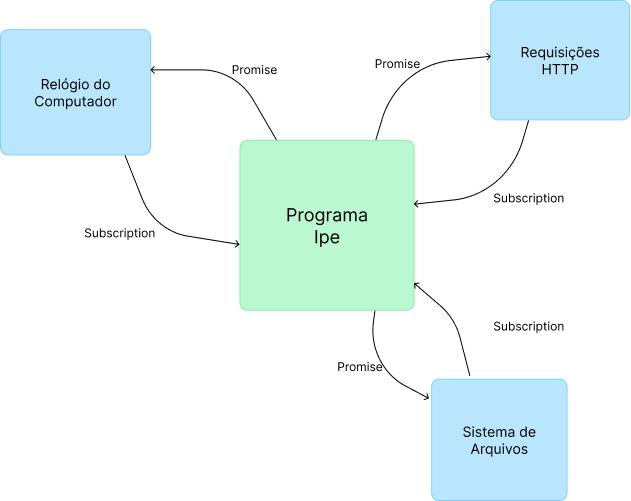
\includegraphics[scale=0.65]{pictures/runtime.png}
    \end{center}
\end{figure}

Para dizer ao \textit{Runtime} quais funções utilizar como funções de inicialização,
\textit{update} e \textit{subscribe}, programas Ipe devem exportar uma função \texttt{main} do módulo
apontado como módulo de entrada (geralmente \texttt{Root.ipe}). O \autoref{lst:full-program} mostra
um exemplo de programa completo em Ipe, que imprime na tela uma mensagem a cada minuto, parando depois
de imprimir 10 vezes.

\begin{lstlisting}[label={lst:full-program},caption={Exemplo de programa completo em Ipe, que imprime na tela uma mensagem a cada minuto}]
module Root exports [main]

type alias Model = { messagesPrinted : Number }

type union Event = 
    | PrintMessage
    | PrintedMessage (Result Console.Error String)

main : { init : { model : Model, effect : Effect Event }
       , update : Event -> Model -> { model : Model, effect : Effect Event }
       , subscribe : Model -> Subscription Event
       }
main =
    { init = { model = { messagesPrinted = 0 }, effect = Effect.none }
    , update = update
    , subscribe = subscribe
    }

update : Event -> Model -> { model : Model, effect : Effect Event }
update =
    \event model ->
        match event with
            | PrintMessage ->
                { model = model
                , effect = 
                    String.fromInt model.messagesPrinted
                    |> Console.log
                    |> Promise.perform PrintedMessage
                }
            | PrintedMessage ->
                { model =
                    { messagesPrinted = model.messagesPrinted + 1 }
                , effect = Effect.none
                }

subscribe : Model -> Subscription Event
subscribe =
    \model ->
        match Number.compare model.messagesPrinted 10 with
            | Number.Smaller -> Time.every 60000 PrintMessage
            | Number.Equal -> Subscription.none
            | Number.Greater -> Subscription.none
\end{lstlisting}

Os passos que o \textit{Runtime} toma para executar o \autoref{lst:full-program}
são:

\begin{enumerate}
    \item Ler a função \texttt{main} para saber quais são as funções \texttt{init},
          \texttt{update} e \texttt{subscribe}.
    \item Executa a função \texttt{init}, e define o estado inicial do programa
          como o \texttt{Record} \texttt{\{ messagesPrinted = 0 \}}. Caso a função \texttt{init}
          retornasse um efeito colateral, o \textit{Runtime} executaria o efeito colateral.
    \item Usa o modelo inicial para executar a função \texttt{subscribe}, e
          começa a esperar por eventos.
    \item Quando um evento chega, o \textit{Runtime} executa a função \texttt{update}
          com o evento e o modelo atual. Efeitos (retornados pelas funções \texttt{init}
          e \texttt{update}) também produzem eventos, que também são tratados na função
          \texttt{update}. Após cada chamada a \texttt{update}, a função \texttt{subscribe}
          é chamada novamente.
    \item Após imprimir 10 vezes na tela, a função \texttt{subscribe} retorna
          \texttt{Subscription.none}, e o programa para de esperar por eventos.
          Quando não existem mais efeitos sendo processados, e a função \texttt{subscribe}
          retorna \texttt{Subscription.none}, o programa termina.
\end{enumerate}

A \autoref{fig:runtime-internals} mostra mais detalhes de como as funções \texttt{init},
\texttt{update} e \texttt{subscribe} se integram com o \textit{Runtime}.

\begin{figure}[htb]
    \caption{Arquitetura detalhada do \textit{Runtime} Ipe}
    \label{fig:runtime-internals}
    \begin{center}
        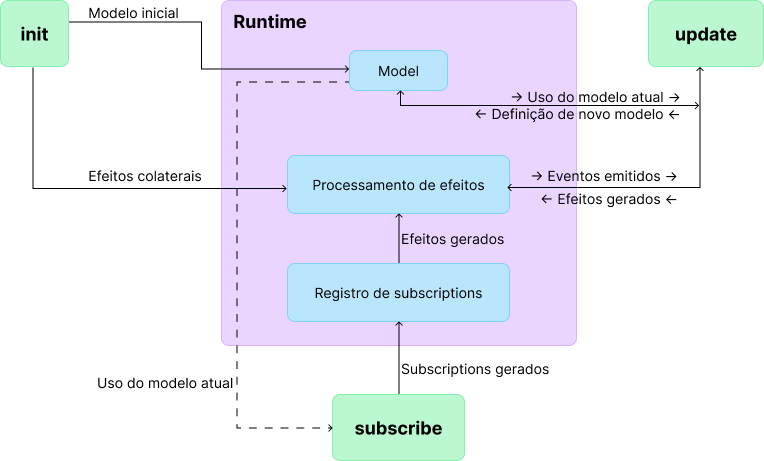
\includegraphics[scale=0.5]{pictures/runtime-internals.png}
    \end{center}
\end{figure}

Podemos ver que, após a definição do modelo inicial em \texttt{init}, as funções
\texttt{update} e \texttt{subscribe} leem o modelo, e respondem a eventos.

Embora este seja o fluxo principal de execução, alguns módulos do \textit{Prelude} de Ipe podem oferecer
funções auxiliares, que ajudam a definir o comportamento do programa, de maneira mais apropriada de
acordo com uma certa necessidade ou contexto. Por exemplo, com \texttt{Http.createApp}, o modelo
passa a se chamar contexto, a função \texttt{init} se chama \texttt{createContext}, e a função
\texttt{update} é substituída pela função \texttt{handleRequest}, de forma que algumas partes do
funcionamento do servidor são omitidas do programador final, como a \texttt{Subscription} que escuta
por requisições HTTP, ou o efeito que envia respostas HTTP.


\phantomsection

\chapter{Cronograma}
\phantomsection

Até agora, já analisamos algumas outras linguagens, e colhemos inspirações para
o desenvolvimento de Ipe. Usamos estas informações no \autoref{chapter:specification}
para definir a linguagem Ipe. Agora, vamos nos concentrar na implementação da
linguagem de fato. Para tal, usaremos a linguagem de programação Haskell.  A
\autoref{tab:cronograma} descreve os próximos passos para o desenvolvimento de Ipe.

\begin{table}[htb]
    \caption{Cronograma de desenvolvimento para a linguagem Ipe}
    \label{tab:cronograma}
    \resizebox{\textwidth}{!}{%
        \begin{tabular}{p{9.5cm}p{4.65cm}}
            \toprule
            \textbf{Tarefa}                                             & \textbf{Tempo estimado para conclusão} \\
            \midrule
            \textit{Parsing} de código fonte                            & 2 semanas                              \\
            Checagem de tipos                                           & 1 semana                               \\
            Geração de código Javascript                                & 1 semana                               \\
            Construção do \textit{Runtime} e módulos padrão             & 3 semanas                              \\
            Construção da aplicação base em Ipe e análise de resultados & 2 semanas                              \\
            \bottomrule
        \end{tabular}
    }
\end{table}

Ao todo, estima-se que o desenvolvimento da linguagem Ipe levará cerca de mais 9
semanas, ou seja, 63 dias.


\phantomsection

\chapter{Conclusões finais}
\phantomsection

Este trabalho apresenta Ipe, uma linguagem de programação puramente funcional.
Ipe visa usar características de linguagens e \textit{frameworks} de desenvolvimento
de aplicações \textit{backend} modernos. Vimos algumas dessas características na
\autoref{subsec:js} e \autoref{subsec:python}, quando vimos aplicações \textit{backend}
em Javascript e Python, respectivamente. Também vimos o exemplo de uma aplicação
em Haskell, na \autoref{subsec:haskell}, e vimos que, embora o código seja bastante
resiliente, ele é extremamente complexo e difícil de compreender. Ipe tem o objetivo
de simplificar o uso da programação funcional, sem comprometer a expressividade
garantida por linguagens funcionais e diminuindo a barreira de entrada no mundo
funcional, seguindo o exemplo de Elm.

No \autoref{chapter:specification}, definimos as características e a sintaxe da
linguagem Ipe: vimos definições de módulos, tipos e funções. Também discutimos
sobre a arquitetura e o \textit{runtime} Ipe no \autoref{chapter:programas-em-ipe},
que possibilitam programas compostos apenas de funções puras, sem efeitos colaterais,
mas que sejam úteis no mundo real.

Nos próximos capítulos a serem escritos, iremos discutir sobre a implementação
de Ipe, usando a linguagem de programação Haskell, uma das principais linguagens
funcionais. Também iremos construir o \textit{runtime} Ipe, junto com alguns módulos
padrão que serão usados em todos os programas Ipe.

Até o momento, concluímos os objetivos específicos 1, 2 e 3 (definidos na
\autoref{sec:objectives}). Assim que tivermos a linguagem, o \textit{runtime} e
os módulos padrão em mãos, podemos construir a aplicação base descrita na
\autoref{sec:aplicacao-base} em Ipe, para que possamos comparar essa implementação
com as que fizemos no \autoref{chapter:trabalhos-relacionados} e verificar se
atingimos o restante dos objetivos.


% ELEMENTOS PÓS-TEXTUAIS
\postextual
\setlength\beforechapskip{0pt}
\setlength\midchapskip{15pt}
\setlength\afterchapskip{15pt}

% Referências bibliográficas
\begingroup
% https://tex.stackexchange.com/questions/163559/how-to-modify-line-spacing-per-entry-of-bibliography
% https://tex.stackexchange.com/questions/19105/how-can-i-put-more-space-between-bibliography-entries-biblatex
\setlength\bibitemsep{\baselineskip}
\advisor{}{\linespread{1.18}\selectfont}

% https://tex.stackexchange.com/questions/17128/using-bibtex-to-make-a-list-of-references-without-having-citations-in-the-body
% \nocite{*}
\printbibliography[title=\lang{REFERENCES}{REFERÊNCIAS}]
\endgroup

% % Inicia os apêndices
\begin{apendicesenv}
    % Imprime uma página indicando o início dos apêndices
    \ifforcedinclude\else\partapendices\fi
    \setlength\beforechapskip{50pt}
    \setlength\midchapskip{20pt}
    \setlength\afterchapskip{20pt}

    \chapter{Descrição completa da sintaxe de Ipe em EBNF}
\label{apendix:ebnf-syntax}

Neste apêndice, apresentamos a sintaxe completa de
Ipe usando a notação EBNF, de acordo com \cite{ebnfstandard} (como iremos fazer
o nosso próprio \textit{parser}-- ao invés de usar um gerador automático --a
gramática não será otimizada-- as ferramentas que usaremos para construir o
\textit{parser} fazem isso por nós --, e alguns detalhes não serão apresentados,
como espaços em branco e comentários de bloco entre tokens). O símbolo inicial
da gramática é \texttt{file}. Discutimos mais sobre a sintaxe de Ipe no
\autoref{chapter:specification}.

\begin{bnfgrammar}
    file ::= module, \{new type $\vert$ tl value\}-;
    ;;
    line comment ::= "\slash\slash", \{? qualquer caractere ?\} - "\textbackslash n", "\textbackslash n";
    ;;
    block comment ::= "\slash*", \{? qualquer caractere ?\} - "*\slash", "*\slash";
    ;;
    doc comment ::= "\slash*$\vert$", \{? qualquer caractere ?\} - "*\slash", "*\slash";
    ;;
    upper identifier ::= uppercase letter, \{letter $\vert$ digit $\vert$ "\_"\};
    ;;
    lower identifier ::= lowercase letter, \{letter $\vert$ digit $\vert$ "\_"\};
    ;;
    number ::= ["$-$"], \{digit\}-, [".", \{digit\}-];
    ;;
    string ::= "'", \{? qualquer caractere ?\} - ("\textbackslash n" $\vert$ "'"), "'";
    ;;
    module name ::= \{upper identifier, "."\}, upper identifier;
    ;;
    exported item ::= letter, \{letter $\vert$ digit $\vert$ "\_"\};
    ;;
    export list ::= "[", \{exported item\}-, "]";
    ;;
    module decl ::= "module", module name, "exports", export list;
    ;;
    import decl ::= "import", module name, [ "as", module name ];
    ;;
    module ::= module decl, [doc comment], \{import decl\};
    ;;
    field decl ::= lower identifier, "$\colon$", expression;
    ;;
    record ::= "\{", [field decl, \{",", field decl\}], "\}";
    ;;
    custom type ::= \{upper identifier, "."\}, upper identifier, \{any type\};
    ;;
    any type ::= custom type
    | lower identifier
    | record annotation;
    ;;
    record ann field ::= lower identifier, "$\colon$", any type;
    ;;
    record annotation ::= "\{", [record ann field, \{",", record ann field\}] "\}";
    ;;
    alias ::= upper identifier, parameters, "=", any type;
    ;;
    union ::= upper identifier, parameters, "=", \{constructor\}-;
    ;;
    constructor ::= "$\vert$", upper identifier, [record annotation];
    ;;
    new type ::= "type alias", alias
    | "type union", union
    | "type opaque", union;
\end{bnfgrammar}
\begin{bnfgrammar}
    fn args ::= \{lowercase identifier\};
    ;;
    function ::= "\textbackslash", fn args, "$-$>", \{attribution\}, expression;
    ;;
    tl annotation ::= lowercase identifier, "$\colon$", \{any type, "$-$>"\}, any type;
    ;;
    attribution ::= lowercase identifier, "$=$", expression;
    ;;
    tl left ::= [doc comment], [tl annotation], lowercase identifier;
    ;;
    tl value ::= tl left "$=$", expression;
    ;;
    type destruct ::= \{upper identifier, "."\}, upper identifier, \{pattern\};
    ;;
    pattern ::= "\_"
    | number
    | string
    | type destruct;
    ;;
    match case ::= "$\vert$", pattern, "$-$>", \{attribution\}, expression;
    ;;
    match ::= "match", expression, "with", \{match case\}-;
    ;;
    expression ::= expression, "$\vert$>", expression
    | expression, "$<$$\vert$", expression
        | function
        | match
        | exponentiation;
        ;;
        exponentiation ::= exponentiation, "\textasciicircum", term
        | term;
        ;;
        term ::= term, ("+" $\vert$ "$-$"), factor
        | factor;
        ;;
        factor ::= factor, ("\slash" $\vert$ "*"), primary
    | primary;
    ;;
    primary ::= number
    | string
    | record
    | variable name, \{primary\}
    | "(", expression, ")";
    ;;
    variable name ::= \{uppercase identifier, "."\}, record access;
    ;;
    record access ::= lowercase identifier, ".", record access
    | lowercase identifier;
\end{bnfgrammar}

\end{apendicesenv}

% TODO - Adicionar anexos
% % Inicia os anexos
% \begin{anexosenv}
%     % Imprime uma página indicando o início dos anexos
%     \ifforcedinclude\else\partanexos\fi
%     \setlength\beforechapskip{50pt}
%     \setlength\midchapskip{20pt}
%     \setlength\afterchapskip{20pt}

%     

%
% How to fix the Underfull \vbox badness has occurred while \output is active on my memoir chapter style?
% https://tex.stackexchange.com/questions/387881/how-to-fix-the-underfull-vbox-badness-has-occurred-while-output-is-active-on-m
%

% ----------------------------------------------------------
\chapter{\lang{Article published in SOBRAEP magazine}{Artigo publicado}}
% ----------------------------------------------------------


% Multiple-language document - babel - selectlanguage vs begin/end{otherlanguage}
% https://tex.stackexchange.com/questions/36526/multiple-language-document-babel-selectlanguage-vs-begin-endotherlanguage
\begin{otherlanguage*}{english}

% An environment for setting \emergencystretch locally
% https://tex.stackexchange.com/questions/84510/an-environment-for-setting-emergencystretch-locally
{
    \setlength{\emergencystretch}{10pt}
    \section[English guidelines for publication]
    {English guidelines for publication - TITLE HERE (14 PT TYPE SIZE, UPPERCASE, BOLD, CENTERED)}
}
    \noindent\textbf{Abstract:}
    The objective of this document is to instruct the authors about the preparation of the
    manuscript for its submission to the Revista Eletrônica de Potência (Brazilian Power Electronics
    Journal).~The authors should use these guidelines for preparing both the initial and final
    versions of their paper. Additional information about procedures and guidelines for publication
    can be obtained directly with the editor, or through the web site
    \url{http://www.sobraep.org.br/revista}. This text was written according to these guidelines

\end{otherlanguage*}

% What is a “Overfull \hbox (9.89561pt too wide)”?
% https://tex.stackexchange.com/questions/111948/what-is-a-overfull-hbox-9-89561pt-too-wide
interwordspace: \the\fontdimen2\font

interwordstretch: \the\fontdimen3\font

emergencystretch: \the\emergencystretch\par\relax


\modifiedincludepdf{-}{ArtigoSOBRAEP}{pictures/SOBRAEP.pdf}{0.9}



%     


%
% How to fix the Underfull \vbox badness has occurred while \output is active on my memoir chapter style?
% https://tex.stackexchange.com/questions/387881/how-to-fix-the-underfull-vbox-badness-has-occurred-while-output-is-active-on-m
%

% ----------------------------------------------------------
\lang
{\chapter[Sample example]{How to display the font size in use in the final output}}
{\chapter[Anexo exemplo]{Como exibir o tamanho da fonte em uso na saída final}}
% ----------------------------------------------------------


% Multiple-language document - babel - selectlanguage vs begin/end{otherlanguage}
% https://tex.stackexchange.com/questions/36526/multiple-language-document-babel-selectlanguage-vs-begin-endotherlanguage
\begin{otherlanguage*}{english}

\showfont

1. How to display the font size in use in the final output,
2. How to display the font size in use in the final output,
3. How to display the font size in use in the final output,


\section[Some encoding tests]{\showfont}

1. How to display the font size in use in the final output,
2. How to display the font size in use in the final output,
3. How to display the font size in use in the final output,
4. How to display the font size in use in the final output,
5. How to display the font size in use in the final output,
6. How to display the font size in use in the final output,

7. How to display the font size in use in the final output,
8. How to display the font size in use in the final output,
9. How to display the font size in use in the final output,
10. How to display the font size in use in the final output,
11. How to display the font size in use in the final output,
12. How to display the font size in use in the final output,

\subsection{\showfont}

1. How to display the font size in use in the final output,
2. How to display the font size in use in the final output,
3. How to display the font size in use in the final output,
4. How to display the font size in use in the final output,
5. How to display the font size in use in the final output,
6. How to display the font size in use in the final output,

7. How to display the font size in use in the final output,
8. How to display the font size in use in the final output,
9. How to display the font size in use in the final output,
10. How to display the font size in use in the final output,
11. How to display the font size in use in the final output,
12. How to display the font size in use in the final output,

\subsubsection{\showfont}

1. How to display the font size in use in the final output,
2. How to display the font size in use in the final output,
3. How to display the font size in use in the final output,
4. How to display the font size in use in the final output,
5. How to display the font size in use in the final output,
6. How to display the font size in use in the final output,

7. How to display the font size in use in the final output,
8. How to display the font size in use in the final output,
9. How to display the font size in use in the final output,
10. How to display the font size in use in the final output,
11. How to display the font size in use in the final output,
12. How to display the font size in use in the final output,

\subsubsubsection{\showfont}

1. How to display the font size in use in the final output,
2. How to display the font size in use in the final output,
3. How to display the font size in use in the final output,
4. How to display the font size in use in the final output,
5. How to display the font size in use in the final output,
6. How to display the font size in use in the final output,
7. How to display the font size in use in the final output,

8. How to display the font size in use in the final output,
9. How to display the font size in use in the final output,
10. How to display the font size in use in the final output,
11. How to display the font size in use in the final output,
12. How to display the font size in use in the final output,


Lipsum me [55-65]

\end{otherlanguage*}



% \end{anexosenv}

\end{document}

